%%%%%%%%%%%%%%%%%%%%%%%%%%%%%%%%%%%%%%%%%%%%%%%%%%%%%%%%%%%%%%%%%%
%%%%%%%%%%%%%%%%%%%%%%%%%%%%%%%%%%%%%%%%%%%%%%%%%%%%%%%%%%%%%%%%%%
%Packages
\documentclass[10pt, a4paper]{article}
\usepackage[top=3cm, bottom=4cm, left=3.5cm, right=3.5cm]{geometry}
\usepackage{amsmath,amsthm,amsfonts,amssymb,amscd, fancyhdr, color, comment, graphicx, environ}

\usepackage{float}
\usepackage{mathrsfs}
\usepackage[math-style=ISO]{unicode-math}
\setmathfont{TeX Gyre Termes Math}
\usepackage{lastpage}
\usepackage[dvipsnames]{xcolor}
\usepackage[framemethod=TikZ]{mdframed}
\usepackage{enumerate}
\usepackage[shortlabels]{enumitem}
\usepackage{fancyhdr}
\usepackage{indentfirst}
\usepackage{listings}
\usepackage{sectsty}
\usepackage{thmtools}
\usepackage{shadethm}
\usepackage{hyperref}
\usepackage{setspace}
\hypersetup{
    colorlinks=true,
    linkcolor=blue,
    filecolor=magenta,      
    urlcolor=blue,
}
\usepackage[makeroom]{cancel}
\usepackage[utf8]{inputenc}
\usepackage[T1]{fontenc}
\usepackage{hyperref}
\hypersetup{colorlinks=true, linkcolor=blue, filecolor=magenta, urlcolor=cyan,}
\urlstyle{same}
\usepackage{amsmath}
\usepackage{amsfonts}
\usepackage{amssymb}
\usepackage[version=4]{mhchem}
\usepackage{stmaryrd}
\usepackage{graphicx}
\usepackage{subcaption}
\usepackage{pgffor}
\usepackage[export]{adjustbox}
\graphicspath{ {./images/} }
\usepackage{listings}
%%%%%%%%%%%%%%%%%%%%%%%%%%%%%%%%%%%%%%%%%%%%%%%%%%%%%%%%%%%%%%%%%%
%%%%%%%%%%%%%%%%%%%%%%%%%%%%%%%%%%%%%%%%%%%%%%%%%%%%%%%%%%%%%%%%%%
%Environment setup
\mdfsetup{skipabove=\topskip,skipbelow=\topskip}
\newrobustcmd\ExampleText{%
An \textit{inhomogeneous linear} differential equation has the form
\begin{align}
L[v ] = f,
\end{align}
where $L$ is a linear differential operator, $v$ is the dependent
variable, and $f$ is a given non−zero function of the independent
variables alone.
}
\mdfdefinestyle{theoremstyle}{%
linecolor=black,linewidth=1pt,%
frametitlerule=true,%
frametitlebackgroundcolor=gray!20,
innertopmargin=\topskip,
}
\mdtheorem[style=theoremstyle]{Problem}{Problem}
\newenvironment{Solution}{\textbf{Solution.}}

\definecolor{codegreen}{rgb}{0,0.6,0}
\definecolor{codegray}{rgb}{0.5,0.5,0.5}
\definecolor{codepurple}{rgb}{0.58,0,0.82}
\definecolor{backcolour}{rgb}{0.95,0.95,0.92}

\lstdefinestyle{mystyle}{
    backgroundcolor=\color{backcolour},   
    commentstyle=\color{codegreen},
    keywordstyle=\color{magenta},
    numberstyle=\tiny\color{codegray},
    stringstyle=\color{codepurple},
    basicstyle=\ttfamily\footnotesize,
    breakatwhitespace=false,         
    breaklines=true,                 
    captionpos=b,                    
    keepspaces=true,                 
    numbers=left,                    
    numbersep=5pt,                  
    showspaces=false,                
    showstringspaces=false,
    showtabs=false,                  
    tabsize=2
}

\lstset{style=mystyle}
%%%%%%%%%%%%%%%%%%%%%%%%%%%%%%%%%%%%%%%%%%%%%%%%%%%%%%%%%%%%%%%%%%
%%%%%%%%%%%%%%%%%%%%%%%%%%%%%%%%%%%%%%%%%%%%%%%%%%%%%%%%%%%%%%%%%%
%Fill in the appropriate information below
\newcommand{\norm}[1]{\left\lVert#1\right\rVert}     
\newcommand\course{CS5785}                            % <-- course name   
\newcommand\hwnumber{4}                                 % <-- homework number
\newcommand\Information{Arystan Tatishev, Maanas Peri}                        % <-- personal information
%%%%%%%%%%%%%%%%%%%%%%%%%%%%%%%%%%%%%%%%%%%%%%%%%%%%%%%%%%%%%%%%%%
%%%%%%%%%%%%%%%%%%%%%%%%%%%%%%%%%%%%%%%%%%%%%%%%%%%%%%%%%%%%%%%%%%
%Page setup
\pagestyle{fancy}
\headheight 35pt
\lhead{\today}
\rhead{
\includegraphics[width=2.5cm]{logo-ct.png}}
\lfoot{}
\pagenumbering{arabic}
\cfoot{\small\thepage}
\rfoot{}
\headsep 1.2em
\renewcommand{\baselinestretch}{1.25}
%%%%%%%%%%%%%%%%%%%%%%%%%%%%%%%%%%%%%%%%%%%%%%%%%%%%%%%%%%%%%%%%%%
%%%%%%%%%%%%%%%%%%%%%%%%%%%%%%%%%%%%%%%%%%%%%%%%%%%%%%%%%%%%%%%%%%
%Add new commands here
\renewcommand{\labelenumi}{\alph{enumi})}
\newcommand{\Z}{\mathbb Z}
\newcommand{\R}{\mathbb R}
\newcommand{\Q}{\mathbb Q}
\newcommand{\NN}{\mathbb N}
\newcommand{\PP}{\mathbb P}
\DeclareMathOperator{\Mod}{Mod} 
\renewcommand\lstlistingname{Algorithm}
\renewcommand\lstlistlistingname{Algorithms}
\def\lstlistingautorefname{Alg.}
\newtheorem*{theorem}{Theorem}
\newtheorem*{lemma}{Lemma}
\newtheorem{case}{Case}
\newcommand{\assign}{:=}
\newcommand{\infixiff}{\text{ iff }}
\newcommand{\nobracket}{}
\newcommand{\backassign}{=:}
\newcommand{\tmmathbf}[1]{\ensuremath{\boldsymbol{#1}}}
\newcommand{\tmop}[1]{\ensuremath{\operatorname{#1}}}
\newcommand{\tmtextbf}[1]{\text{{\bfseries{#1}}}}
\newcommand{\tmtextit}[1]{\text{{\itshape{#1}}}}

\newenvironment{itemizedot}{\begin{itemize} \renewcommand{\labelitemi}{$\bullet$}\renewcommand{\labelitemii}{$\bullet$}\renewcommand{\labelitemiii}{$\bullet$}\renewcommand{\labelitemiv}{$\bullet$}}{\end{itemize}}
\catcode`\<=\active \def<{
\fontencoding{T1}\selectfont\symbol{60}\fontencoding{\encodingdefault}}
\catcode`\>=\active \def>{
\fontencoding{T1}\selectfont\symbol{62}\fontencoding{\encodingdefault}}
\catcode`\<=\active \def<{
\fontencoding{T1}\selectfont\symbol{60}\fontencoding{\encodingdefault}}

%%%%%%%%%%%%%%%%%%%%%%%%%%%%%%%%%%%%%%%%%%%%%%%%%%%%%%%%%%%%%%%%%%
%%%%%%%%%%%%%%%%%%%%%%%%%%%%%%%%%%%%%%%%%%%%%%%%%%%%%%%%%%%%%%%%%%
%Begin now!



\begin{document}

\begin{titlepage}
    \begin{center}
        \vspace*{3cm}
            
        \Huge
        \textbf{Assignment}
            
        \vspace{1cm}
        \huge
        Homework \hwnumber
            
        \vspace{1.5cm}
        \Large
            
        \textbf{\Information}                      % <-- author
        
            
        \vfill
        
        A \course \ Homework Assignment
            
        \vspace{1cm}
            
        
\includegraphics[width=0.4\textwidth]{logo-ct.png}
        \\
        
        \Large
        
        \today
            
    \end{center}
\end{titlepage}

%%%%%%%%%%%%%%%%%%%%%%%%%%%%%%%%%%%%%%%%%%%%%%%%%%%%%%%%%%%%%%%%%%
%%%%%%%%%%%%%%%%%%%%%%%%%%%%%%%%%%%%%%%%%%%%%%%%%%%%%%%%%%%%%%%%%%
%Start the assignment now
%%%%%%%%%%%%%%%%%%%%%%%%%%%%%%%%%%%%%%%%%%%%%%%%%%%%%%%%%%%%%%%%%%
%New problem
\newpage
\section*{Programming Exercises}
\section{Convolutional Neural Networks}
In this problem, you will implement several machine learning techniques from the class to perform classification on text data. Throughout the problem, we will be working on the NLP with Disaster Tweets Kaggle competition, where the task is to predict whether or not a tweet is about a real disaster.

\begin{lstlisting}[language=Python]
import keras
keras . __version__
\end{lstlisting}

The above lines will give you the current version of Keras you are using. Once this works, you can proceed with the assignment.

\begin{Problem*}[(a) Loading Dataset]
For using this dataset, you will need to import mnist and use it as follows.

\begin{lstlisting}[language=Python]
from keras.datasets import mnist
(train_X, train_Y), (test_X, test_Y) = mnist.load_data()
\end{lstlisting}

To verify that you have loaded the dataset correctly, try printing out the shape of your train and test dataset matrices. Also, try to visualize individual images in this dataset by using imshow() function in pyplot. Below are some example images from the Tensorflow datasets catalog.

\end{Problem*}

\begin{Solution}
\begin{lstlisting}[language=Python]
import matplotlib.pyplot as plt

# Shapes of the datasets
print('Training data shape : ', train_X.shape, train_Y.shape)
print('Testing data shape : ', test_X.shape, test_Y.shape)

# Visualize the first image in the training dataset
plt.imshow(train_X[0], cmap='gray')
plt.title('First image in the training dataset')
plt.show()

for i in range(10):
    plt.subplot(1, 10, i + 1)  # Creates a subplot for each image
    plt.imshow(train_X[i], cmap='gray')  # Replace 'gray' with 'viridis' if your images are in color
    plt.axis('off')  # Turns off the axis

plt.show()

# Visualize the first image in the test dataset
plt.imshow(test_X[0], cmap='gray')
plt.title('First image in the test dataset')
plt.show()

for i in range(10):
    plt.subplot(1, 10, i + 1)  # Creates a subplot for each image
    plt.imshow(test_X[i], cmap='gray')  # Replace 'gray' with 'viridis' if your images are in color
    plt.axis('off')  # Turns off the axis

plt.show()
\end{lstlisting}

Training data shape :  (60000, 28, 28) (60000,)
Testing data shape :  (10000, 28, 28) (10000,)

\begin{figure}[H]
    \centering
    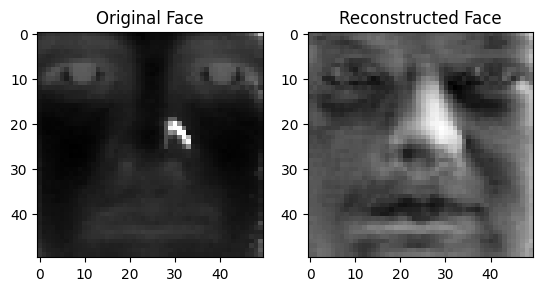
\includegraphics[width=0.5\linewidth]{HW4//images/image5.png}
    \caption{First image in the training dataset}
    \label{fig:enter-label}
\end{figure}

\begin{figure}[H]
    \centering
    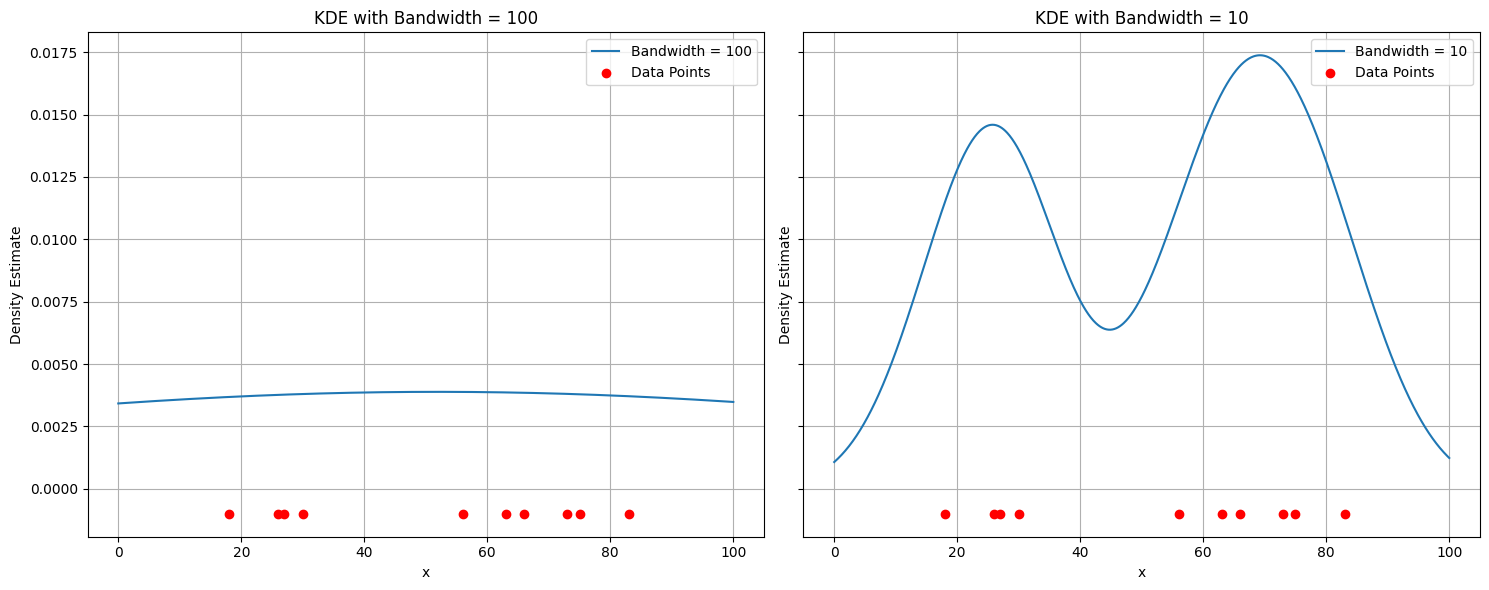
\includegraphics[width=0.5\linewidth]{HW4//images/image6.png}
    \caption{First image in the test dataset}
    \label{fig:enter-label}
\end{figure}

\end{Solution}

\begin{Problem*}[(b) Preprocessing]
The data has images with $28 \times 28$ pixel values. Since we use just one grayscale color channel, you need to reshape the matrix such that we have a $28 \times 28 \times 1$ sized matrix holding each input data-point in the training and testing dataset. The output variable can be converted into a one-hot vector by using the function to\_categorical (make sure you import to\_categorical from keras.utils). For example, if the output label for a given image is the digit 2 , then the one-hot representation for this consists of a 10 -element vector, where the element at index 2 is set to 1 and all the other elements are zero.

For preprocessing, scale the pixel values such that they lie between 0.0 and 1.0. Make sure that you use the appropriate conversion to float wherever required while scaling.

You can include all these steps into a single python function that loads your dataset appropriately. Once you finish this, visualize some images using imshow() function.
\end{Problem*}

\begin{Solution}
\begin{lstlisting}[language=Python]
# Import necessary components for preprocessing
from keras.utils import to_categorical
import numpy as np

# Function to load and preprocess the data
def load_and_preprocess_mnist(train_X, train_Y, test_X, test_Y):

    # Reshape dataset to have a single channel
    train_X = train_X.reshape((train_X.shape[0], 28, 28, 1))
    test_X = test_X.reshape((test_X.shape[0], 28, 28, 1))

    # Convert from integers to floats and normalize to range 0-1
    train_X = train_X.astype('float32') / 255.0
    test_X = test_X.astype('float32') / 255.0

    # Convert the labels to one-hot vectors
    train_Y = to_categorical(train_Y)
    test_Y = to_categorical(test_Y)

    return (train_X, train_Y), (test_X, test_Y)

# Load and preprocess the data
(train_x, train_y), (test_x, test_y) = load_and_preprocess_mnist(train_X, train_Y, test_X, test_Y)

# Check the shape after preprocessing
print('Training data shape : ', train_x.shape, train_y.shape)
print('Testing data shape : ', test_x.shape, test_y.shape)

# Visualize some images after preprocessing
fig, axes = plt.subplots(1, 5, figsize=(15, 3))
for i, ax in enumerate(axes):
    ax.imshow(train_x[i].reshape(28, 28), cmap='gray')
    ax.set_title('Label: {}'.format(np.argmax(train_y[i])))
    ax.axis('off')
plt.show()
\end{lstlisting}

Training data shape :  (60000, 28, 28, 1) (60000, 10)
Testing data shape :  (10000, 28, 28, 1) (10000, 10)

\begin{figure}[H]
    \centering
    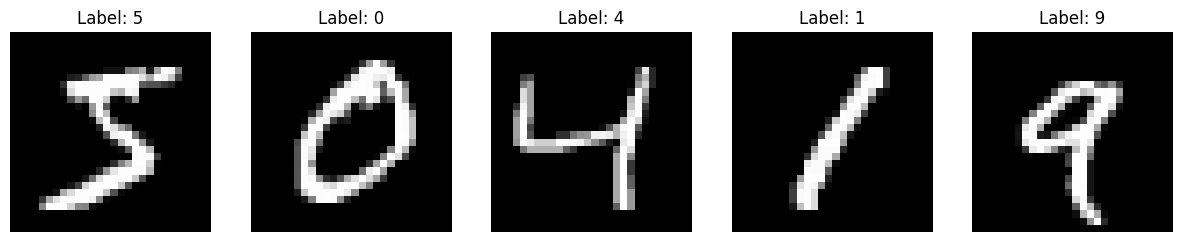
\includegraphics[width=1\linewidth]{HW4//images/image7.png}
    \caption{Visualize some images after preprocessing}
    \label{fig:enter-label}
\end{figure}
\end{Solution}

\begin{Problem*}[(c) Implementation]
Now, to define a CNN model, we will use the Sequential module in Keras. We are providing you with the code for creating a simple CNN here. We use Conv2D (for declaring 2D convolutional networks), MaxPooling2D (for maxpooling layer), Dense (for densely connected neural network layers) and Flatten (for flattening the input for next layer).

\begin{lstlisting}[language=Python]
from keras.models import Sequential
from keras.layers import Conv2D
from keras.layers import MaxPooling2D
from keras.layers import Dense
from keras.layers import Flatten
from keras.optimizers import SGD

def create_cnn():
    # define using Sequential
    model = Sequential()
    # Convolution layer
    model.add(
        Conv2D(32, (3, 3),
        activation='relu',
        kernel_initializer='he_uniform',
        input_shape=(28, 28, 1))
    )
    # Maxpooling layer
    model.add(MaxPooling2D((2, 2)))
    # Flatten output
    model.add(Flatten())
    # Dense layer of 100 neurons
    model.add(
        Dense(100,
        activation='relu',
        kernel_initializer='he_uniform')
    )
    model.add(Dense(10, activation='softmax'))
    # initialize optimizer
    opt = SGD(lr=0.01, momentum=0.9)
    # compile model
    model.compile(
        optimizer=opt,
        loss='categorical_crossentropy',
        metrics=['accuracy']
    )
    return model
\end{lstlisting}
Specifically, we have added the following things in this code.
\begin{enumerate}
    \item A single convolutional layer with $3 \times 3$ sized window for computing the convolution, with 32 filters
    \item Maxpooling layer with $2 \times 2$ window size.
    \item Flatten resulting features to reshape your output appropriately.
    \item Dense layer on top of this (100 neurons) with ReLU activation
    \item Dense layer with 10 neurons for calculating softmax output (Our classification result will output one of the ten possible classes, corresponding to our digits)
\end{enumerate}
After defining this model, we use Stochastic Gradient Descent (SGD) optimizer and crossentropy loss to compile the model. We are using a learning rate of 0.01 and a momentum of 0.9 here. We have added this to the given code stub already. Please see that this code stub works for you. Try to print model.layers in your interactive shell to see that the model is generated as we defined.
\end{Problem*}

\begin{Solution}
\begin{lstlisting}[language=Python]
# Create the CNN model
model = create_cnn()

# Print the model layers
for layer in model.layers:
    print(layer)
\end{lstlisting}
<keras.src.layers.convolutional.conv2d.Conv2D object at 0x7e020a1294b0> \\
<keras.src.layers.pooling.max_pooling2d.MaxPooling2D object at 0x7e021750ee90> \\
<keras.src.layers.reshaping.flatten.Flatten object at 0x7e021750c220> \\
<keras.src.layers.core.dense.Dense object at 0x7e020a159bd0> \\
<keras.src.layers.core.dense.Dense object at 0x7e020a1583d0> \\
\end{Solution}

\begin{Problem*}[(d) Training and Evaluating CNN]
Now we will train the network. You can see some examples here. Look at the fit() and evaluate() methods.

You will call the fit method with a validation split of 0.1 (i.e. $10 \%$ of data will be used for validation in every epoch). Please use 10 epochs and a batch size of 32 . When you evaluate the trained model, you can call the evaluate method on the test data-set. Please report the accuracy on test data after you have trained it as above. You can refer to the following while you write code for training and evaluating your CNN.

\begin{lstlisting}[language=Python]
model.fit(train_x, train_y, batch_size=32, epochs=10, validation_split=0.1)
score = model.evaluate(test_x, test_y, verbose=0)
print(f"Test accuracy: {score[1]*100:.2f}%")
\end{lstlisting}
\end{Problem*}

\begin{Solution}
\begin{figure}[H]
    \centering
    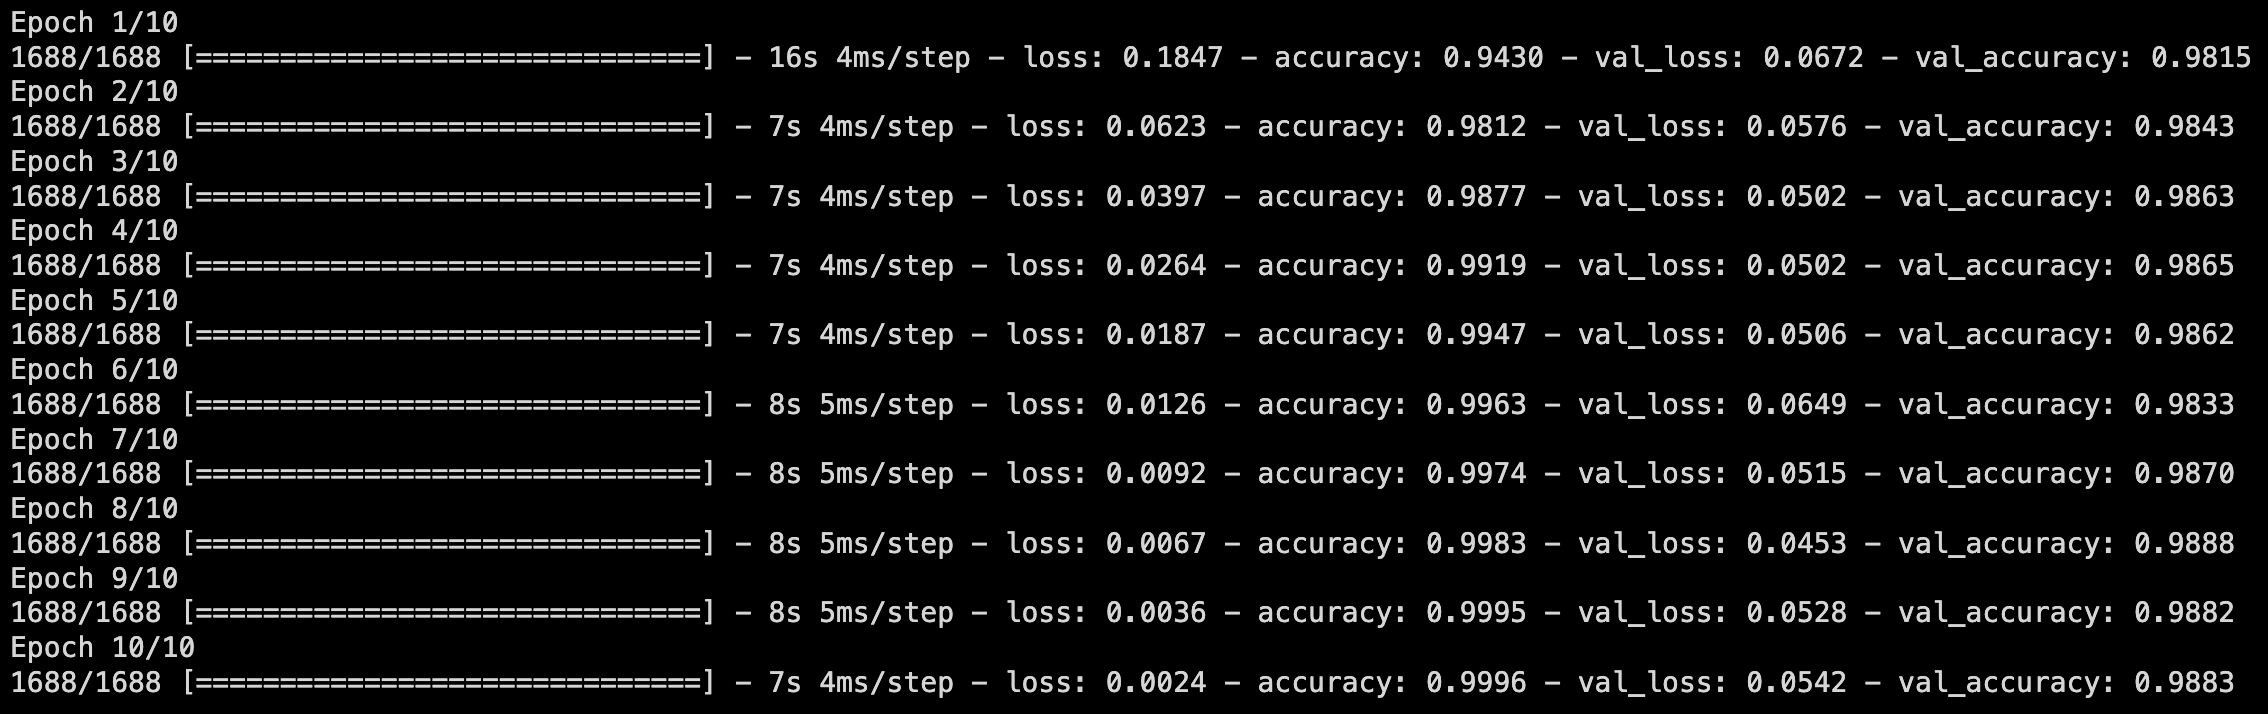
\includegraphics[width=1\linewidth]{HW4//images/image10.png}
    \caption{10 Epochs}
    \label{fig:enter-label}
\end{figure}
Test accuracy: 98.83%
\end{Solution}

\begin{Problem*}[(e) Experimentation]
 
\end{Problem*}

\begin{Problem*}[i. Run the above training for 50 epochs.]
 Using pyplot, graph the validation and training accuracy after every 10 epochs. Is there a steady improvement for both training and validation accuracy?

For accessing the required values while plotting, you can store the output of the fit method while training your network. Please refer to the code below.
\end{Problem*}

\begin{Solution}
\begin{lstlisting}[language=Python]
# Training and validation accuracy
train_acc = epoch_history.history['accuracy']
val_acc = epoch_history.history['val_accuracy']

# Print training and validation accuracy
print("Training accuracy after each epoch:")
print(train_acc)
print("\nValidation accuracy after each epoch:")
print(val_acc)

# Ensure you have 50 points to plot for both training and validation
assert len(train_acc) == 50 and len(val_acc) == 50, "The training and validation lists should each have 50 elements."

# Plot training & validation accuracy values
plt.figure(figsize=(12, 6))
plt.plot(range(1, 51), train_acc, 'b', label='Training Accuracy')
plt.plot(range(1, 51), val_acc, 'r', label='Validation Accuracy')
plt.xticks(range(0, 51, 10))
plt.title('Training and Validation Accuracy over Epochs')
plt.xlabel('Epochs')
plt.ylabel('Accuracy')
plt.legend()
plt.show()
\end{lstlisting}
\begin{figure}
    \centering
    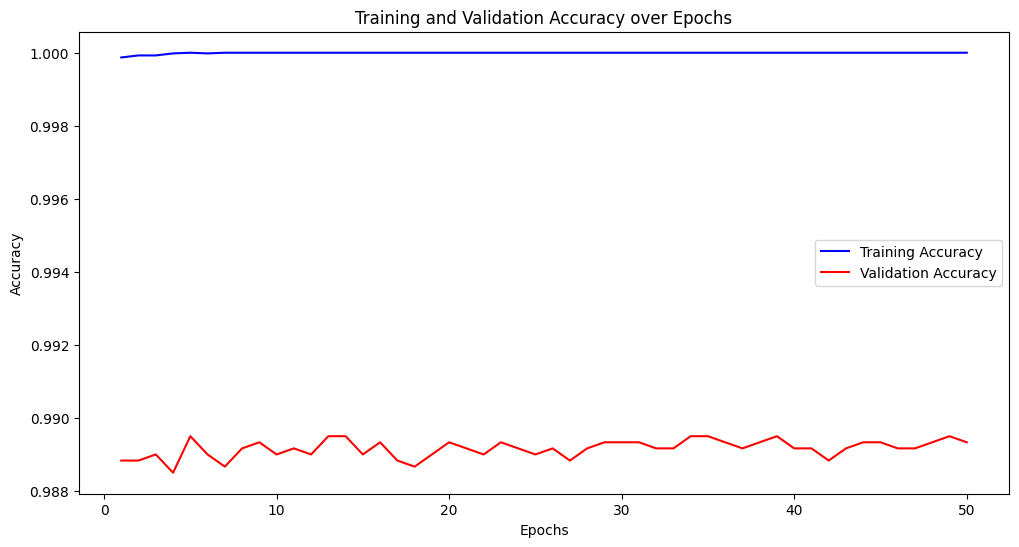
\includegraphics[width=1\linewidth]{HW4//images/image8.png}
    \caption{Training and Validation Accuracy over Epochs}
    \label{fig:enter-label}
\end{figure}
\end{Solution}

\begin{Problem*}[ii. To avoid over-fitting in neural networks, we can 'drop out' a certain fraction of units randomly during the training phase.]
You can add the following layer (before the dense layer with 100 neurons) to your model defined in the function create\_cnn.

\begin{lstlisting}[language=Python]
model.add(Dropout(0.5))
\end{lstlisting}
Make sure you import Dropout from keras.layers! Now, train this CNN for 50 epochs.

Graph the validation and train accuracy after every 10 epochs.

This tutorial might be helpful if you want to see more examples of dropout with Keras.
\end{Problem*}

\begin{Solution}
\begin{lstlisting}[language=Python]
from keras.layers import Dropout

def create_cnn_with_dropout():
    # define using Sequential
    model = Sequential()
    # Convolution layer
    model.add(
        Conv2D(32, (3, 3),
        activation='relu',
        kernel_initializer='he_uniform',
        input_shape=(28, 28, 1))
    )
    # Maxpooling layer
    model.add(MaxPooling2D((2, 2)))
    # Flatten output
    model.add(Flatten())
    # Dropout layer added
    model.add(Dropout(0.5))
    # Dense layer of 100 neurons
    model.add(
        Dense(100,
        activation='relu',
        kernel_initializer='he_uniform')
    )
    model.add(Dense(10, activation='softmax'))
    # initialize optimizer
    opt = SGD(learning_rate=0.01, momentum=0.9)
    # compile model
    model.compile(
        optimizer=opt,
        loss='categorical_crossentropy',
        metrics=['accuracy']
    )
    return model

# Create the CNN with dropout
model_with_dropout = create_cnn_with_dropout()

# Train the CNN with dropout for 50 epochs
history_with_dropout = model_with_dropout.fit(train_x, train_y, batch_size=32, epochs=50, validation_split=0.1)

# Extract training and validation accuracy
train_acc_with_dropout = history_with_dropout.history['accuracy']
val_acc_with_dropout = history_with_dropout.history['val_accuracy']

# Plot training & validation accuracy values
plt.figure(figsize=(12, 6))
plt.plot(range(1, 51), train_acc_with_dropout, 'b', label='Training Accuracy with Dropout')
plt.plot(range(1, 51), val_acc_with_dropout, 'r', label='Validation Accuracy with Dropout')
plt.xticks(range(0, 51, 10))
plt.title('Training and Validation Accuracy with Dropout over Epochs')
plt.xlabel('Epochs')
plt.ylabel('Accuracy')
plt.legend()
plt.show()
\end{lstlisting}

\begin{figure}[H]
    \centering
    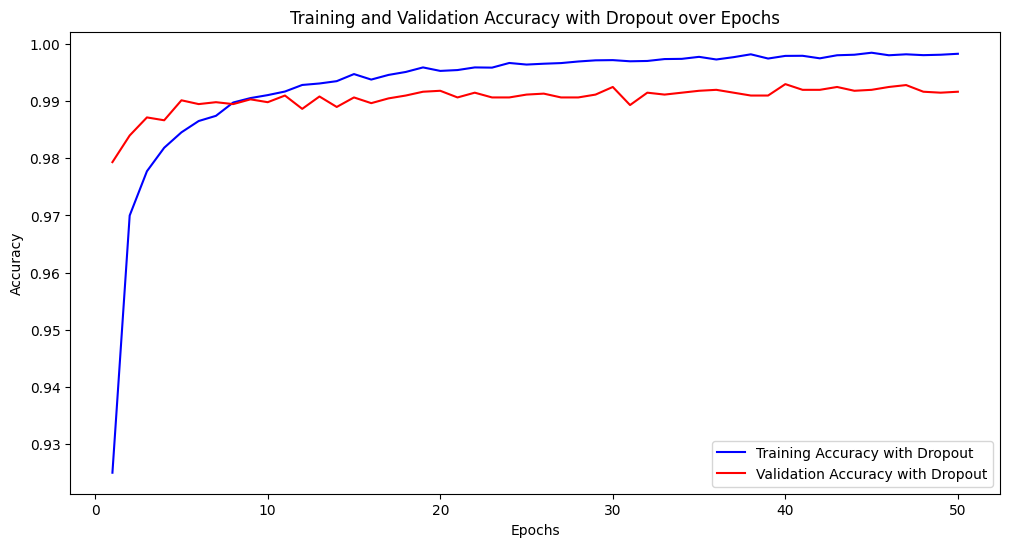
\includegraphics[width=1\linewidth]{HW4//images/image9.png}
    \caption{Training and Validation Accuracy with Dropout over Epochs}
    \label{fig:enter-label}
\end{figure}

\end{Solution}

\begin{Problem*}[iii. Add another convolution layer and maxpooling layer to the create\_cnn function defined above (immediately following the existing maxpooling layer).]

For the additional convolution layer, use 64 output filters. Train this for 10 epochs and report the test accuracy.
\end{Problem*}

\begin{Solution}
\begin{lstlisting}[language=Python]
def create_cnn_with_dropout_extra_layers():
    # define using Sequential
    model = Sequential()
    # Convolution layer
    model.add(
        Conv2D(32, (3, 3),
        activation='relu',
        kernel_initializer='he_uniform',
        input_shape=(28, 28, 1))
    )
    # Maxpooling layer
    model.add(MaxPooling2D((2, 2)))
    # New Convolution layer with 64 filters
    model.add(Conv2D(64, (3, 3), activation='relu', kernel_initializer='he_uniform'))
    # New MaxPooling layer
    model.add(MaxPooling2D((2, 2)))
    # Flatten output
    model.add(Flatten())
    # Dropout layer added
    model.add(Dropout(0.5))
    # Dense layer of 100 neurons
    model.add(
        Dense(100,
        activation='relu',
        kernel_initializer='he_uniform')
    )
    model.add(Dense(10, activation='softmax'))
    # initialize optimizer
    opt = SGD(learning_rate=0.01, momentum=0.9)
    # compile model
    model.compile(
        optimizer=opt,
        loss='categorical_crossentropy',
        metrics=['accuracy']
    )
    return model

# Create the updated CNN model with extra layers
updated_model = create_cnn_with_dropout_extra_layers()

# Train the updated CNN model for 10 epochs
updated_model.fit(train_x, train_y, batch_size=32, epochs=10, validation_split=0.1)

# Evaluate the model on the test data
test_loss, test_accuracy = updated_model.evaluate(test_x, test_y, verbose=0)

print(f"Test accuracy: {test_accuracy*100:.2f}%")
\end{lstlisting}

Test accuracy: 99.13\%

\end{Solution}

\begin{Problem*}[iv. We used a learning rate of 0.01 in the given create\_cnn function.]

Using learning rates of 0.001 and 0.1 respectively, train the model and report accuracy on test data-set. Use Dropout, 2 convolution layers and train for 10 epochs for this experiment.
\end{Problem*}

\begin{Solution}
\begin{lstlisting}[language=Python]
def create_cnn_with_dropout_extra_layers_custom_lr(lr):
    # define using Sequential
    model = Sequential()
    # Convolution layer
    model.add(
        Conv2D(32, (3, 3),
        activation='relu',
        kernel_initializer='he_uniform',
        input_shape=(28, 28, 1))
    )
    # Maxpooling layer
    model.add(MaxPooling2D((2, 2)))
    # New Convolution layer with 64 filters
    model.add(
        Conv2D(64, (3, 3),
        activation='relu',
        kernel_initializer='he_uniform',
        input_shape=(28, 28, 1))
    )
    # New MaxPooling layer
    model.add(MaxPooling2D((2, 2)))
    # Flatten output
    model.add(Flatten())
    # Dropout layer added
    model.add(Dropout(0.5))
    # Dense layer of 100 neurons
    model.add(
        Dense(100,
        activation='relu',
        kernel_initializer='he_uniform')
    )
    model.add(Dense(10, activation='softmax'))
    # initialize optimizer
    opt = SGD(learning_rate=lr, momentum=0.9)
    # compile model
    model.compile(
        optimizer=opt,
        loss='categorical_crossentropy',
        metrics=['accuracy']
    )
    return model

# Create the updated CNN model with learning rate of 0.001
lr_0001_model = create_cnn_with_dropout_extra_layers_custom_lr(0.001)

# Train the updated CNN models for 10 epochs
lr_0001_model.fit(train_x, train_y, batch_size=32, epochs=10, validation_split=0.1)

# Evaluate the model on the test data
test_loss_0001, test_accuracy_0001 = lr_0001_model.evaluate(test_x, test_y, verbose=0)

print(f"Test accuracy (learning rate of 0.001): {test_accuracy_0001*100:.2f}%")
\end{lstlisting}

Test accuracy (learning rate of 0.001): 98.74\%

\begin{lstlisting}[language=Python]
# Create the updated CNN model with learning rate of 0.001
lr_0001_model = create_cnn_with_dropout_extra_layers_custom_lr(0.001)

# Train the updated CNN models for 10 epochs
lr_0001_model.fit(train_x, train_y, batch_size=32, epochs=10, validation_split=0.1)

# Evaluate the model on the test data
test_loss_0001, test_accuracy_0001 = lr_0001_model.evaluate(test_x, test_y, verbose=0)

print(f"Test accuracy (learning rate of 0.001): {test_accuracy_0001*100:.2f}%")
\end{lstlisting}

Test accuracy (learning rate of 0.1): 10.28\%

\end{Solution}

\begin{Problem*}[(f) Analysis]
\end{Problem*}

\begin{Problem*}[i.]
 Explain how the trends in validation and train accuracy change after using the dropout layer in the experiments.
\end{Problem*}

\begin{Solution}
In the first experiment without dropout, the training accuracy is very high, remaining close to 100\% throughout the epochs. The validation accuracy, although high, is somewhat volatile and consistently lower than the training accuracy, indicating a gap that could suggest overfitting; the model is performing better on the training data than on the validation data.

When dropout is introduced in the second experiment, the following changes are observed:

\begin{itemize}
    \item Training Accuracy with Dropout: The training accuracy starts lower compared to the non-dropout scenario, which is expected because dropout randomly ignores a portion of neurons during the training phase, effectively providing a form of regularization. This helps in preventing the model from fitting too closely to the training data. Over the epochs, the training accuracy increases steadily but doesn't reach as high as in the non-dropout scenario, again due to the regularization effect of dropout.
    \item Validation Accuracy with Dropout: The validation accuracy improves compared to the non-dropout scenario and shows less volatility. It starts lower but quickly rises and remains close to the training accuracy, indicating that the model is generalizing better to unseen data. The gap between training and validation accuracy has reduced significantly, suggesting that the model is less overfitted than the model without dropout.
\end{itemize}: 

Dropout is intended to reduce overfitting by preventing complex co-adaptations on training data. It forces the model to learn more robust features that are useful in conjunction with many different random subsets of the other neurons. The model with dropout is less likely to rely on any small set of neurons and thus becomes more capable of better generalization. This is evident from the fact that the validation accuracy is closer to the training accuracy, which suggests that the model is learning patterns that are more representative of the underlying data distribution, rather than memorizing the training data.
\end{Solution}

\begin{Problem*}[ii.]
 How does the performance of CNN with two convolution layers differ as compared to CNN with a single convolution layer in your experiments?
\end{Problem*}

\begin{Solution}
It's expected that adding another convolution layer will make the model able to learn more complex information. It's almost as if the first layer learns basic patterns, and then the second layer learns intricate details along with the combination of general patterns. Too many layers will introduce lots of parameters, which can also be prone to overfitting. These are the tradeoffs an engineer has to make.
\end{Solution}

\begin{Problem*}[iii.]
 How did changing learning rates change your experimental results in part (iv)?
\end{Problem*}

\begin{Solution}
Changing the learning rates in our experiments had a significant impact on the results:

\begin{enumerate}
    \item Learning Rate of 0.001:
    \begin{itemize}
        \item With a lower learning rate of 0.001, the model likely learned more gradually. It made smaller updates to the weights, which generally helps in finding a more stable and possibly better local minimum in the loss function. This can be particularly beneficial when the model is complex and there's a risk of overshooting the optimal points in the loss landscape.
        \item The test accuracy you achieved with this learning rate was quite high (98.74\%), suggesting that the model was able to generalize well from the training data to the unseen test data. This indicates that for the given architecture and dataset, a learning rate of 0.001 was effective.
    \end{itemize}
    \item Learning Rate of 0.1:
    \begin{itemize}
        \item On the other hand, a much higher learning rate of 0.1 likely caused the model's training process to be too aggressive. With large updates to the weights, the model might have failed to converge and missed the finer details necessary for accurate predictions, as it could not settle into a more precise minimum of the loss function.
        \item The test accuracy plummeted to 10.28\%, which is close to a random guess accuracy for a 10-class classification problem (which would be 10%). This suggests that the model did not learn effectively and was not better than random guessing.
    \end{itemize}
\end{enumerate}

In summary, the learning rate controls how quickly or slowly a neural network model learns from the training data. A learning rate that is too low may result in a very slow training process, while a learning rate that is too high can cause the model to converge too quickly to a suboptimal solution, or even fail to converge at all. In our case, the lower learning rate of 0.001 helped the model in converging to a solution that generalizes well to unseen data, whereas the higher learning rate of 0.1 was too high for the model to learn anything meaningful.
\end{Solution}

\section{Random Forests for Image Approximation}

In this question, you will use random forest regression to approximate an image by learning a function, $f: \mathbb{R}^{2} \rightarrow \mathbb{R}$, that takes image $(x, y)$ coordinates as input and outputs pixel brightness. This way, the function learns to approximate areas of the image that it has not seen before.

\begin{Problem*}[a. Start with an image of the Mona Lisa.]
If you don't like the Mona Lisa, pick another interesting image of your choice.
\end{Problem*}

\begin{Solution}
\begin{lstlisting}[language=Python]

from google.colab import drive
drive.mount('/content/drive')

mona_lisa = '/content/drive/MyDrive/AML_HW4/Mona_Lisa,_by_Leonardo_da_Vinci,_from_C2RMF_retouched.jpg'

\end{lstlisting}
\end{Solution}

\begin{Problem*}[b. Preprocessing the input.]
To build your "training set," uniformly sample 5,000 random $(x, y)$ coordinate locations.

What other preprocessing steps are necessary for random forests inputs? Describe them, implement them, and justify your decisions. In particular, do you need to perform mean subtraction, standardization, or unit-normalization?
\end{Problem*}

\begin{Solution}
\begin{lstlisting}[language=Python]

import numpy as np
from PIL import Image
import random
import matplotlib.pyplot as plt

# Load the image
# img = Image.open(mona_lisa) # .convert('L')  # Convert to grayscale if needed
img = Image.open(mona_lisa).convert('RGB')  # Convert to RGB if needed

plt.imshow(img)
plt.axis('off')  # To turn off the axis
plt.show()

\end{lstlisting}

\begin{figure}[H]
    \centering
    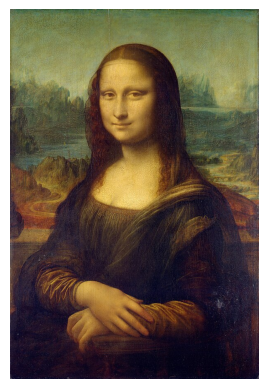
\includegraphics[width=0.5\linewidth]{HW4/images/mona_lisa.png}
    \label{fig:enter-label}
\end{figure}

\begin{lstlisting}[language=Python]
#Before normalization, checking min and max pixels
print(np.min(img), np.max(img))
#Normalization
img = np.array(img) / 255.0

plt.imshow(img)
plt.show()

print(np.min(img), np.max(img))
\end{lstlisting}


\begin{figure}[H]
    \centering
    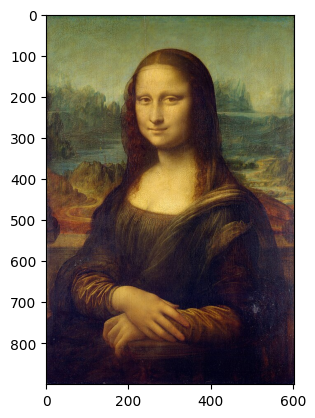
\includegraphics[width=0.5\linewidth]{HW4/images/mona_lisa_2.png}
    \label{fig:enter-label}
\end{figure}
Output: 
0.0 1.0


Preprocessing steps I took:

Extracting Pixel Brightness: For each sampled (x, y) coordinate, you need to extract the pixel brightness. If the image is in grayscale, the brightness is the pixel value itself. If the image is in color, you may convert it to grayscale or take the brightness as the intensity of one of the RGB channels or a combination of them (like the luminance component in the YUV color space).

Normalizing Pixel Brightness: Normalizing the pixel brightness values to a range such as [0, 1] can be beneficial, especially if you are dealing with a color image with multiple channels to ensure that all output values are on a consistent scale.

Mean Subtraction and Standardization: Unlike methods such as neural networks, random forests do not require input features to be zero-centered or standardized because they are not sensitive to the scale of the features. Decision trees in the forest make decisions by thresholding feature values, and these thresholds are learned from the data. Therefore, mean subtraction (making the data zero-centered) and standardization (scaling the data to have unit variance) are not necessary preprocessing steps for random forests.

\end{Solution}

\begin{Problem*}[c. Preprocessing the output.]
Sample pixel values at each of the given coordinate locations. Each pixel contains red, green, and blue intensity values, so decide how you want to handle this. \\
There are several options available to you:
  \item Convert the image to grayscale

  \item Regress all three values at once, so your function maps $(x, y)$ coordinates to $(r, g, b)$ values: $f: \mathbb{R}^{2} \rightarrow \mathbb{R}^{3}$

  \item Learn a different function for each channel, $f_{\text {Red }}: \mathbb{R}^{2} \rightarrow \mathbb{R}$, and likewise for $f_{\text {Green }}, f_{\text {Blue }}$.

Note that you may need to rescale the pixel intensities to lie between 0.0 and 1.0. (The default for pixel values may be between 0 and 255, but your image library may have different defaults.)

What other preprocessing steps are necessary for random regression forest outputs? Describe them, implement them, and justify your decisions.
\end{Problem*}

\begin{Solution}

#Cited Sources: Used gpt to generate comments and debug initial faulty images

One of the preprocessing steps of the output we took was scaling coordinates.

It is common to scale the input coordinates to a standard range, typically [0, 1], especially if the random forest implementation you are using performs any distance-based computations. This ensures that the coordinate system of the image does not unduly influence the learning process.

Other steps included rescaling the pixel intensities and using the regressed coordinates to handle rgb channels

\begin{lstlisting}


# Get image dimensions
height, width, channels = img.shape

num_samples = 5000
sampled_x = np.random.randint(0, width, size=num_samples)
sampled_y = np.random.randint(0, height, size=num_samples)
# print(sampled_x)

# Normalize coordinates
sampled_coordinates = np.stack((sampled_x, sampled_y), axis=1) / np.array([width, height]) # Rescaled pixel intensities to 0, 1
print(np.min(sampled_coordinates), np.max(sampled_coordinates))
#Output: 0.0 0.9988888888888889 as expected. 


# Assuming `img` is your original image
plt.imshow(img)

# Scatter plot the sampled coordinates
plt.scatter(sampled_x, sampled_y, c='red', marker='.', s=5)

# Show the plot
plt.show()
print(sampled_coordinates)

# Assuming 'image' is a numpy array of shape (height, width, channels)
sampled_pixels = img[sampled_y, sampled_x] #/ 255.0  # Already Rescaled the SAMPLED PIXELS to [0, 1] as mentioned above 

# made sure that the regressed values are compartmentalized to handle the handled 3 rgb channels below
\end{lstlisting}

\begin{figure}[H]
    \centering
    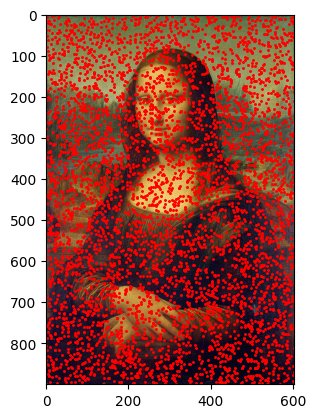
\includegraphics[width=0.5\linewidth]{HW4/images/mona_lisa_red_dot.png}
    \label{fig:enter-label}
\end{figure}
\end{Solution}

\begin{Problem*}[d. Final Image]
To build the final image, for each pixel of the output, feed the pixel coordinate through the random forest and color the resulting pixel with the output prediction.
You can then use imshow to view the result. (If you are using grayscale, try imshow ( $Y, c m a p=$ 'gray') to avoid fake-coloring). You may use any implementation of random forests, but you should understand the implementation and you must cite your sources.
\end{Problem*}

\begin{Solution}
\begin{lstlisting}[language=Python]

#Cited Sources:

from sklearn.ensemble import RandomForestRegressor

# Initialize the Random Forest regressors. You could use one regressor for each color channel.
forest_r = RandomForestRegressor(n_estimators=10)
forest_g = RandomForestRegressor(n_estimators=10)
forest_b = RandomForestRegressor(n_estimators=10)

# Split your sampled pixels into R, G, and B components
sampled_pixels_r = sampled_pixels[:, 0]  # Red channel
sampled_pixels_g = sampled_pixels[:, 1]  # Green channel
sampled_pixels_b = sampled_pixels[:, 2]  # Blue channel

# Train the Random Forest model for each color channel
forest_r.fit(sampled_coordinates, sampled_pixels_r)
forest_g.fit(sampled_coordinates, sampled_pixels_g)
forest_b.fit(sampled_coordinates, sampled_pixels_b)

# Predicting the pixel values for each coordinate in the image (for the whole image grid)
# Create a grid of coordinates (for the entire image)
xx, yy = np.meshgrid(np.linspace(0, 1, width), np.linspace(0, 1, height))
flat_grid = np.c_[xx.ravel(), yy.ravel()]

# Predict the pixel values using the trained models
predicted_pixels_r = forest_r.predict(flat_grid)
predicted_pixels_g = forest_g.predict(flat_grid)
predicted_pixels_b = forest_b.predict(flat_grid)

# Re-scale the predicted pixel values to [0, 255]
predicted_pixels_r = (predicted_pixels_r * 255).astype(np.uint8)
predicted_pixels_g = (predicted_pixels_g * 255).astype(np.uint8)
predicted_pixels_b = (predicted_pixels_b * 255).astype(np.uint8)

# Combine the R, G, and B predictions to form the final image
predicted_image = np.stack((predicted_pixels_r, predicted_pixels_g, predicted_pixels_b), axis=-1)
predicted_image = predicted_image.reshape((height, width, 3))

# Display the image
plt.imshow(predicted_image)
plt.axis('off')
plt.show()

\end{lstlisting}

\begin{figure}[H]
    \centering
    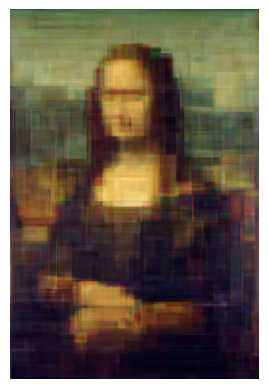
\includegraphics[width=0.5\linewidth]{HW4/images/Mona_lisa_pixelated.png}
    \label{fig:enter-label}
\end{figure}

\begin{lstlisting}
# Output the minimum and maximum of the predicted values
print('Red channel predictions range: min =', predicted_pixels_r.min(), ', max =', predicted_pixels_r.max())
print('Green channel predictions range: min =', predicted_pixels_g.min(), ', max =', predicted_pixels_g.max())
print('Blue channel predictions range: min =', predicted_pixels_b.min(), ', max =', predicted_pixels_b.max())

# Check the standard deviation to assess variance
print('Standard deviation of predictions - Red:', np.std(predicted_pixels_r))
print('Standard deviation of predictions - Green:', np.std(predicted_pixels_g))
print('Standard deviation of predictions - Blue:', np.std(predicted_pixels_b))

\end{lstlisting}
Output: 
Red channel predictions range: min = 2 , max = 245

Green channel predictions range: min = 0 , max = 214

Blue channel predictions range: min = 6 , max = 128

Standard deviation of predictions - Red: 52.13433620846846

Standard deviation of predictions - Green: 50.94945494918122

Standard deviation of predictions - Blue: 23.003095942503627

\end{Solution}

\begin{Problem*}[e. Experimentation]
\end{Problem*}

\begin{Problem*}[i. Repeat the experiment for a random forest containing a single decision tree, but with depths 1, 2, 3, 5, 10, and 15.]
How does depth impact the result? Describe in detail why.
\end{Problem*}

\begin{Solution}

#Cited Sources: Used gpt to generate comments and find the best structure to train our forest model and predict pixel values


The depth of a decision tree matters a lot when trying to do image approximation using Random Forests, especially on the performance side. A shallower tree with a smaller depth will result in a simpler model that generalizes well on unseen data but it's not going to be able to reflect detailed patterns on an image.

On the other hand, a higher depth on a random forest tree allows it to record and predict more detailed patterns and complex relationships within the data. This will result in a great accuracy on a training data set.

However, the trade-off is that if a tree has too much depth on a training set, then it will overfit the data and perform poorly when predicting patterns on unseen data. It's almost as if the tree is memorizing information rather than learning. Thus, picking a happy-medium depth is really important when trying to make a model that generalizes well and also displays intricate patterns for most images

\begin{lstlisting}[language=Python]
from sklearn.ensemble import RandomForestRegressor

# Initialize the Random Forest regressors. You could use one regressor for each color channel.
forest_r = RandomForestRegressor(n_estimators=10, max_depth = 1)
forest_g = RandomForestRegressor(n_estimators=10, max_depth = 1)
forest_b = RandomForestRegressor(n_estimators=10, max_depth = 1)

# Split your sampled pixels into R, G, and B components
sampled_pixels_r = sampled_pixels[:, 0]  # Red channel
sampled_pixels_g = sampled_pixels[:, 1]  # Green channel
sampled_pixels_b = sampled_pixels[:, 2]  # Blue channel

# Train the Random Forest model for each color channel
forest_r.fit(sampled_coordinates, sampled_pixels_r)
forest_g.fit(sampled_coordinates, sampled_pixels_g)
forest_b.fit(sampled_coordinates, sampled_pixels_b)

# Predicting the pixel values for each coordinate in the image (for the whole image grid)
# Create a grid of coordinates (for the entire image)
xx, yy = np.meshgrid(np.linspace(0, 1, width), np.linspace(0, 1, height))
flat_grid = np.c_[xx.ravel(), yy.ravel()]

# Predict the pixel values using the trained models
predicted_pixels_r = forest_r.predict(flat_grid)
predicted_pixels_g = forest_g.predict(flat_grid)
predicted_pixels_b = forest_b.predict(flat_grid)

# Re-scale the predicted pixel values to [0, 255]
predicted_pixels_r = (predicted_pixels_r * 255).astype(np.uint8)
predicted_pixels_g = (predicted_pixels_g * 255).astype(np.uint8)
predicted_pixels_b = (predicted_pixels_b * 255).astype(np.uint8)

# Combine the R, G, and B predictions to form the final image
predicted_image = np.stack((predicted_pixels_r, predicted_pixels_g, predicted_pixels_b), axis=-1)
predicted_image = predicted_image.reshape((height, width, 3))

# Display the image
plt.imshow(predicted_image)
plt.axis('off')
plt.show()

\end{lstlisting}

\begin{figure}[H]
    \centering
    
\includegraphics[width=0.5\linewidth]{HW4/images/exp1.png}
    \label{fig:enter-label}
\end{figure}

\begin{lstlisting}
from sklearn.ensemble import RandomForestRegressor

# Initialize the Random Forest regressors. You could use one regressor for each color channel.
forest_r = RandomForestRegressor(n_estimators=10, max_depth = 2)
forest_g = RandomForestRegressor(n_estimators=10, max_depth = 2)
forest_b = RandomForestRegressor(n_estimators=10, max_depth = 2)

# Split your sampled pixels into R, G, and B components
sampled_pixels_r = sampled_pixels[:, 0]  # Red channel
sampled_pixels_g = sampled_pixels[:, 1]  # Green channel
sampled_pixels_b = sampled_pixels[:, 2]  # Blue channel

# Train the Random Forest model for each color channel
forest_r.fit(sampled_coordinates, sampled_pixels_r)
forest_g.fit(sampled_coordinates, sampled_pixels_g)
forest_b.fit(sampled_coordinates, sampled_pixels_b)

# Predicting the pixel values for each coordinate in the image (for the whole image grid)
# Create a grid of coordinates (for the entire image)
xx, yy = np.meshgrid(np.linspace(0, 1, width), np.linspace(0, 1, height))
flat_grid = np.c_[xx.ravel(), yy.ravel()]

# Predict the pixel values using the trained models
predicted_pixels_r = forest_r.predict(flat_grid)
predicted_pixels_g = forest_g.predict(flat_grid)
predicted_pixels_b = forest_b.predict(flat_grid)

# Re-scale the predicted pixel values to [0, 255]
predicted_pixels_r = (predicted_pixels_r * 255).astype(np.uint8)
predicted_pixels_g = (predicted_pixels_g * 255).astype(np.uint8)
predicted_pixels_b = (predicted_pixels_b * 255).astype(np.uint8)

# Combine the R, G, and B predictions to form the final image
predicted_image = np.stack((predicted_pixels_r, predicted_pixels_g, predicted_pixels_b), axis=-1)
predicted_image = predicted_image.reshape((height, width, 3))

# Display the image
plt.imshow(predicted_image)
plt.axis('off')
plt.show()

\end{lstlisting}

\begin{figure}[H]
    \centering
    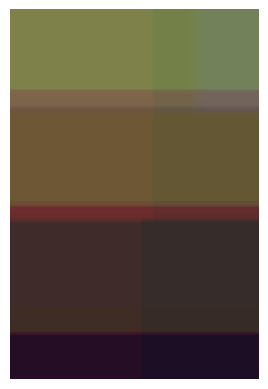
\includegraphics[width=0.5\linewidth]{HW4/images/exp2.png}
    \label{fig:enter-label}
\end{figure}

\begin{lstlisting}
from sklearn.ensemble import RandomForestRegressor

# Initialize the Random Forest regressors. You could use one regressor for each color channel.
forest_r = RandomForestRegressor(n_estimators=10, max_depth = 3)
forest_g = RandomForestRegressor(n_estimators=10, max_depth = 3)
forest_b = RandomForestRegressor(n_estimators=10, max_depth = 3)

# Split your sampled pixels into R, G, and B components
sampled_pixels_r = sampled_pixels[:, 0]  # Red channel
sampled_pixels_g = sampled_pixels[:, 1]  # Green channel
sampled_pixels_b = sampled_pixels[:, 2]  # Blue channel

# Train the Random Forest model for each color channel
forest_r.fit(sampled_coordinates, sampled_pixels_r)
forest_g.fit(sampled_coordinates, sampled_pixels_g)
forest_b.fit(sampled_coordinates, sampled_pixels_b)

# Predicting the pixel values for each coordinate in the image (for the whole image grid)
# Create a grid of coordinates (for the entire image)
xx, yy = np.meshgrid(np.linspace(0, 1, width), np.linspace(0, 1, height))
flat_grid = np.c_[xx.ravel(), yy.ravel()]

# Predict the pixel values using the trained models
predicted_pixels_r = forest_r.predict(flat_grid)
predicted_pixels_g = forest_g.predict(flat_grid)
predicted_pixels_b = forest_b.predict(flat_grid)

# Re-scale the predicted pixel values to [0, 255]
predicted_pixels_r = (predicted_pixels_r * 255).astype(np.uint8)
predicted_pixels_g = (predicted_pixels_g * 255).astype(np.uint8)
predicted_pixels_b = (predicted_pixels_b * 255).astype(np.uint8)

# Combine the R, G, and B predictions to form the final image
predicted_image = np.stack((predicted_pixels_r, predicted_pixels_g, predicted_pixels_b), axis=-1)
predicted_image = predicted_image.reshape((height, width, 3))

# Display the image
plt.imshow(predicted_image)
plt.axis('off')
plt.show()

\end{lstlisting}

\begin{figure}[H]
    \centering
    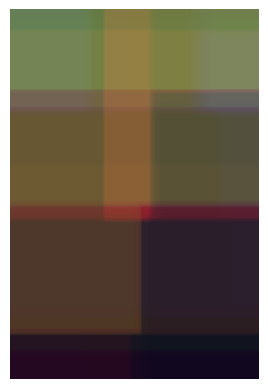
\includegraphics[width=0.5\linewidth]{HW4/images/exp3.png}
    \label{fig:enter-label}
\end{figure}

\begin{lstlisting}
from sklearn.ensemble import RandomForestRegressor

# Initialize the Random Forest regressors. You could use one regressor for each color channel.
forest_r = RandomForestRegressor(n_estimators=10, max_depth = 5)
forest_g = RandomForestRegressor(n_estimators=10, max_depth = 5)
forest_b = RandomForestRegressor(n_estimators=10, max_depth = 5)

# Split your sampled pixels into R, G, and B components
sampled_pixels_r = sampled_pixels[:, 0]  # Red channel
sampled_pixels_g = sampled_pixels[:, 1]  # Green channel
sampled_pixels_b = sampled_pixels[:, 2]  # Blue channel

# Train the Random Forest model for each color channel
forest_r.fit(sampled_coordinates, sampled_pixels_r)
forest_g.fit(sampled_coordinates, sampled_pixels_g)
forest_b.fit(sampled_coordinates, sampled_pixels_b)

# Predicting the pixel values for each coordinate in the image (for the whole image grid)
# Create a grid of coordinates (for the entire image)
xx, yy = np.meshgrid(np.linspace(0, 1, width), np.linspace(0, 1, height))
flat_grid = np.c_[xx.ravel(), yy.ravel()]

# Predict the pixel values using the trained models
predicted_pixels_r = forest_r.predict(flat_grid)
predicted_pixels_g = forest_g.predict(flat_grid)
predicted_pixels_b = forest_b.predict(flat_grid)

# Re-scale the predicted pixel values to [0, 255]
predicted_pixels_r = (predicted_pixels_r * 255).astype(np.uint8)
predicted_pixels_g = (predicted_pixels_g * 255).astype(np.uint8)
predicted_pixels_b = (predicted_pixels_b * 255).astype(np.uint8)

# Combine the R, G, and B predictions to form the final image
predicted_image = np.stack((predicted_pixels_r, predicted_pixels_g, predicted_pixels_b), axis=-1)
predicted_image = predicted_image.reshape((height, width, 3))

# Display the image
plt.imshow(predicted_image)
plt.axis('off')
plt.show()

\end{lstlisting}

\begin{figure}[H]
    \centering
    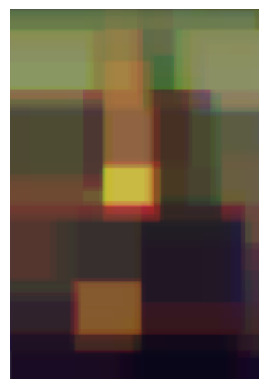
\includegraphics[width=0.5\linewidth]{HW4/images/exp4.png}
    \label{fig:enter-label}
\end{figure}

\begin{lstlisting}
from sklearn.ensemble import RandomForestRegressor

# Initialize the Random Forest regressors. You could use one regressor for each color channel.
forest_r = RandomForestRegressor(n_estimators=10, max_depth = 10)
forest_g = RandomForestRegressor(n_estimators=10, max_depth = 10)
forest_b = RandomForestRegressor(n_estimators=10, max_depth = 10)

# Split your sampled pixels into R, G, and B components
sampled_pixels_r = sampled_pixels[:, 0]  # Red channel
sampled_pixels_g = sampled_pixels[:, 1]  # Green channel
sampled_pixels_b = sampled_pixels[:, 2]  # Blue channel

# Train the Random Forest model for each color channel
forest_r.fit(sampled_coordinates, sampled_pixels_r)
forest_g.fit(sampled_coordinates, sampled_pixels_g)
forest_b.fit(sampled_coordinates, sampled_pixels_b)

# Predicting the pixel values for each coordinate in the image (for the whole image grid)
# Create a grid of coordinates (for the entire image)
xx, yy = np.meshgrid(np.linspace(0, 1, width), np.linspace(0, 1, height))
flat_grid = np.c_[xx.ravel(), yy.ravel()]

# Predict the pixel values using the trained models
predicted_pixels_r = forest_r.predict(flat_grid)
predicted_pixels_g = forest_g.predict(flat_grid)
predicted_pixels_b = forest_b.predict(flat_grid)

# Re-scale the predicted pixel values to [0, 255]
predicted_pixels_r = (predicted_pixels_r * 255).astype(np.uint8)
predicted_pixels_g = (predicted_pixels_g * 255).astype(np.uint8)
predicted_pixels_b = (predicted_pixels_b * 255).astype(np.uint8)

# Combine the R, G, and B predictions to form the final image
predicted_image = np.stack((predicted_pixels_r, predicted_pixels_g, predicted_pixels_b), axis=-1)
predicted_image = predicted_image.reshape((height, width, 3))

# Display the image
plt.imshow(predicted_image)
plt.axis('off')
plt.show()
    
\end{lstlisting}

\begin{figure}[H]
    \centering
    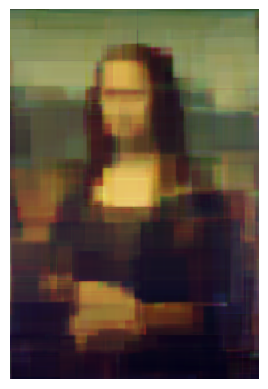
\includegraphics[width=0.5\linewidth]{HW4/images/exp5.png}
    \label{fig:enter-label}
\end{figure}

\end{Solution}

#Cited Sources: Used gpt to generate comments and find the most optimal way to prune different features


\begin{Problem*}[ii. Repeat the experiment for a random forest of depth 7, but with number of trees equal to $1,3,5,10$, and $100$.]
How does the number of trees impact the result? Describe in detail why.
\end{Problem*}
\begin{Solution}

Each tree is called a boostrapped sample because it is independently trained on a subset of the data, with each tree recognizing different general patterns and unique perspectives. Ensemble averaging is the process of averaging up the predictions from each of these trees and smoothen out the predictions. This is useful because it eliminates any outliers or further noise. While increasing the number of the trees improves the ensemble, there is usually a limit where there isn't much added value from each tree added.  

Overall, the number of trees in a Random Forest has a big impact on the performance of the model. As the number of trees increase, the model becomes less likely to overfit and memorize data, which improves the ability to learn and predict accurately on unseen data. However, having too small number of trees might make it more sensitive to particular/random patterns in the data, which is less stable.
\begin{lstlisting}[language=Python]
num_trees_list = [1, 3, 5, 10, 100]

for num_trees in num_trees_list:
    forest_r = RandomForestRegressor(n_estimators=num_trees, max_depth = 7)
    forest_g = RandomForestRegressor(n_estimators=num_trees, max_depth = 7)
    forest_b = RandomForestRegressor(n_estimators=num_trees, max_depth = 7)

    # Split your sampled pixels into R, G, and B components
    sampled_pixels_r = sampled_pixels[:, 0]  # Red channel
    sampled_pixels_g = sampled_pixels[:, 1]  # Green channel
    sampled_pixels_b = sampled_pixels[:, 2]  # Blue channel

    # Train the Random Forest model for each color channel
    forest_r.fit(sampled_coordinates, sampled_pixels_r)
    forest_g.fit(sampled_coordinates, sampled_pixels_g)
    forest_b.fit(sampled_coordinates, sampled_pixels_b)

    # Predicting the pixel values for each coordinate in the image (for the whole image grid)
    # Create a grid of coordinates (for the entire image)
    xx, yy = np.meshgrid(np.linspace(0, 1, width), np.linspace(0, 1, height))
    flat_grid = np.c_[xx.ravel(), yy.ravel()]

    # Predict the pixel values using the trained models
    predicted_pixels_r = forest_r.predict(flat_grid)
    predicted_pixels_g = forest_g.predict(flat_grid)
    predicted_pixels_b = forest_b.predict(flat_grid)

    # Re-scale the predicted pixel values to [0, 255]
    predicted_pixels_r = (predicted_pixels_r * 255).astype(np.uint8)
    predicted_pixels_g = (predicted_pixels_g * 255).astype(np.uint8)
    predicted_pixels_b = (predicted_pixels_b * 255).astype(np.uint8)

    # Combine the R, G, and B predictions to form the final image
    predicted_image = np.stack((predicted_pixels_r, predicted_pixels_g, predicted_pixels_b), axis=-1)
    predicted_image = predicted_image.reshape((height, width, 3))

    # Display the image
    plt.imshow(predicted_image)
    plt.title(f"Random Forest Depth 7, Trees: {num_trees}")
    plt.axis('off')
    plt.show()

\end{lstlisting}

\newcommand{\imgheight}{10cm} % Adjust this value to your preferred height

% Loop for pairs of images
\foreach \n in {21,23}{
    \begin{figure}[H]
        \centering
        \begin{subfigure}{0.48\textwidth}
            \includegraphics[height=\imgheight, width=\linewidth, keepaspectratio]{HW4/images/exp\n.png} 
        \end{subfigure}
        \hfill % This adds space between the images
        \begin{subfigure}{0.48\textwidth}
            \def\m{\number\numexpr\n+1\relax} % Calculate the next image number
            \includegraphics[height=\imgheight, width=\linewidth, keepaspectratio]{HW4/images/exp\m.png} % Adjust the path
        \end{subfigure}
    \end{figure}
}

\begin{figure}[H]
    \centering
    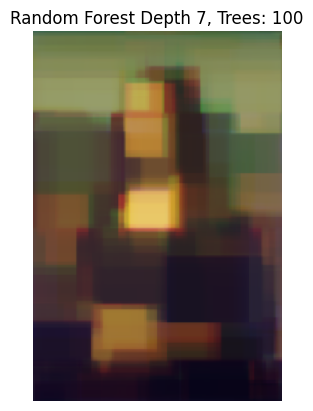
\includegraphics[width=0.5\linewidth]{HW4/images/exp25.png}
    \label{fig:enter-label}
\end{figure}

\end{Solution}

\begin{Problem*}[iii. As a simple baseline, repeat the experiment using a $k$-NN regressor, for $k=1$.]
 This means that every pixel in the output will equal the nearest pixel from the "training set." Compare and contrast the outlook: why does this look the way it does? You may use an existing implementation of $k$-NN but make sure to cite your source.
\end{Problem*}

\begin{Solution}

#Cited Sources: Used gpt to generate comments


In this proposed approach, every pixel in the output will equal the nearest pixel from the training set. Thus, this image will look and feel spotty, with elements of mosiac paintings. This is because the neighboring pixels take on the same color as the randomly sampled points. This means that intricate features are preserved even though there aren't any general patterns that are reproducible unlike the Random Forest Trees. This also means that it's more likely to be affected by noise and outliers, but the image looks way more smooth than the Random Forest Trees. These are the trade-offs.

\begin{lstlisting}[language=Python]
from sklearn.neighbors import KNeighborsRegressor

# Define the number of neighbors (k) for k-NN
k_neighbors = 1

# Initialize the k-NN regressors. You could use one regressor for each color channel.
# Used gpt to debug and understand how this knn used sampled_coordinates and sampled_pixels_r
knn_r = KNeighborsRegressor(n_neighbors=k_neighbors)
knn_g = KNeighborsRegressor(n_neighbors=k_neighbors)
knn_b = KNeighborsRegressor(n_neighbors=k_neighbors)

# Train the k-NN model for each color channel
knn_r.fit(sampled_coordinates, sampled_pixels_r)
knn_g.fit(sampled_coordinates, sampled_pixels_g)
knn_b.fit(sampled_coordinates, sampled_pixels_b)

# Predict the pixel values using the trained models
predicted_pixels_r = knn_r.predict(flat_grid)
predicted_pixels_g = knn_g.predict(flat_grid)
predicted_pixels_b = knn_b.predict(flat_grid)

# Re-scale the predicted pixel values to [0, 255]
predicted_pixels_r = (predicted_pixels_r * 255).astype(np.uint8)
predicted_pixels_g = (predicted_pixels_g * 255).astype(np.uint8)
predicted_pixels_b = (predicted_pixels_b * 255).astype(np.uint8)

# Combine the R, G, and B predictions to form the final image
predicted_image_knn = np.stack((predicted_pixels_r, predicted_pixels_g, predicted_pixels_b), axis=-1)
predicted_image_knn = predicted_image_knn.reshape((height, width, 3))

# Display the image
plt.imshow(predicted_image_knn)
plt.title(f"k-NN Regressor, k={k_neighbors}")
plt.axis('off')
plt.show()

\end{lstlisting}

\begin{figure}[H]
    \centering
    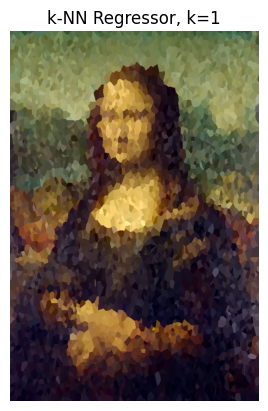
\includegraphics[width=0.5\linewidth]{HW4/images/exp31.png}
    \label{fig:enter-label}
\end{figure}

\end{Solution}

\begin{Problem*}[iv. Further Experimentation]
 Experiment with different pruning strategies of your choice.
\end{Problem*}

\begin{Solution}

\begin{lstlisting}[language=Python]
max_depth_values = [None, 5, 10]
min_samples_leaf_values = [1, 5, 10]
min_samples_split_values = [2, 5, 10]

# Loop through different parameter combinations
for max_d in max_depth_values:
    for min_leaf in min_samples_leaf_values:
        for min_samples_split in min_samples_split_values:
              # Initialize the RandomForestRegressor with pruning parameters
              pruned_forest_r = RandomForestRegressor(n_estimators=10, max_depth = max_d, min_samples_leaf = min_leaf, min_samples_split = min_samples_split)
              pruned_forest_g = RandomForestRegressor(n_estimators=10, max_depth = max_d, min_samples_leaf = min_leaf, min_samples_split = min_samples_split)
              pruned_forest_b = RandomForestRegressor(n_estimators=10, max_depth = max_d, min_samples_leaf = min_leaf, min_samples_split = min_samples_split)

              # Split your sampled pixels into R, G, and B components
              sampled_pixels_r = sampled_pixels[:, 0]  # Red channel
              sampled_pixels_g = sampled_pixels[:, 1]  # Green channel
              sampled_pixels_b = sampled_pixels[:, 2]  # Blue channel

              # Train the Random Forest model for each color channel
              pruned_forest_r.fit(sampled_coordinates, sampled_pixels_r)
              pruned_forest_g.fit(sampled_coordinates, sampled_pixels_g)
              pruned_forest_b.fit(sampled_coordinates, sampled_pixels_b)

              # Predicting the pixel values for each coordinate in the image (for the whole image grid)
              # Create a grid of coordinates (for the entire image)
              xx, yy = np.meshgrid(np.linspace(0, 1, width), np.linspace(0, 1, height))
              flat_grid = np.c_[xx.ravel(), yy.ravel()]

              # Predict the pixel values using the trained models
              predicted_pixels_r = pruned_forest_r.predict(flat_grid)
              predicted_pixels_g = pruned_forest_g.predict(flat_grid)
              predicted_pixels_b = pruned_forest_b.predict(flat_grid)

              # Re-scale the predicted pixel values to [0, 255]
              predicted_pixels_r = (predicted_pixels_r * 255).astype(np.uint8)
              predicted_pixels_g = (predicted_pixels_g * 255).astype(np.uint8)
              predicted_pixels_b = (predicted_pixels_b * 255).astype(np.uint8)

              # Combine the R, G, and B predictions to form the final image
              predicted_image = np.stack((predicted_pixels_r, predicted_pixels_g, predicted_pixels_b), axis=-1)
              predicted_image = predicted_image.reshape((height, width, 3))

              # Display the image
              plt.imshow(predicted_image)
              plt.title(f"Depth: {max_d}, Min_Leaf: {min_leaf} Sample Split: {min_samples_split}")
              plt.axis('off')
              plt.show()

\end{lstlisting}

\newcommand{\imgheight}{10cm} % Adjust this value to your preferred height

% Loop for pairs of images
\foreach \n in {41,43,...,68}{
    \begin{figure}[H]
        \centering
        \begin{subfigure}{0.48\textwidth}
            \includegraphics[height=\imgheight, width=\linewidth, keepaspectratio]{HW4/images/exp\n.png} 
        \end{subfigure}
        \hfill % This adds space between the images
        \begin{subfigure}{0.48\textwidth}
            \def\m{\number\numexpr\n+1\relax} % Calculate the next image number
            \includegraphics[height=\imgheight, width=\linewidth, keepaspectratio]{HW4/images/exp\m.png} % Adjust the path
        \end{subfigure}
    \end{figure}
}

\end{Solution}


\begin{Problem*}[f. Analysis.]
 
\end{Problem*}
\begin{Problem*}[i. What is the decision rule at each split point?]
 Write down the 1-line formula for the split point at the root node for one of the trained decision trees inside the forest. Feel free to define any variables you need.
\end{Problem*}
\begin{Solution}

# Cited Sources: Used gpt to generate comments and find a way to extract the decision boundaries for features of root tree

If X[1] <= 0.5672222077846527, go left; otherwise, go right.

If X[1] <= 0.5338889062404633, go left; otherwise, go right.

If X[1] <= 0.2805555611848831, go left; otherwise, go right.

Plot visualizations for this are displayed below.

\begin{lstlisting}[language=Python]
from sklearn.ensemble import RandomForestRegressor


#Cited Sources:

from sklearn.ensemble import RandomForestRegressor

# Initialize the Random Forest regressors. You could use one regressor for each color channel.
forest_r = RandomForestRegressor(n_estimators=10)
forest_g = RandomForestRegressor(n_estimators=10)
forest_b = RandomForestRegressor(n_estimators=10)

# Split your sampled pixels into R, G, and B components
sampled_pixels_r = sampled_pixels[:, 0]  # Red channel
sampled_pixels_g = sampled_pixels[:, 1]  # Green channel
sampled_pixels_b = sampled_pixels[:, 2]  # Blue channel

# Train the Random Forest model for each color channel
forest_r.fit(sampled_coordinates, sampled_pixels_r)
forest_g.fit(sampled_coordinates, sampled_pixels_g)
forest_b.fit(sampled_coordinates, sampled_pixels_b)

# Predicting the pixel values for each coordinate in the image (for the whole image grid)
# Create a grid of coordinates (for the entire image)
xx, yy = np.meshgrid(np.linspace(0, 1, width), np.linspace(0, 1, height))
flat_grid = np.c_[xx.ravel(), yy.ravel()]

# Predict the pixel values using the trained models
predicted_pixels_r = forest_r.predict(flat_grid)
predicted_pixels_g = forest_g.predict(flat_grid)
predicted_pixels_b = forest_b.predict(flat_grid)

# Re-scale the predicted pixel values to [0, 255]
predicted_pixels_r = (predicted_pixels_r * 255).astype(np.uint8)
predicted_pixels_g = (predicted_pixels_g * 255).astype(np.uint8)
predicted_pixels_b = (predicted_pixels_b * 255).astype(np.uint8)

# Combine the R, G, and B predictions to form the final image
predicted_image = np.stack((predicted_pixels_r, predicted_pixels_g, predicted_pixels_b), axis=-1)
predicted_image = predicted_image.reshape((height, width, 3))

# # Display the image
# plt.imshow(predicted_image)
# plt.axis('off')
# plt.show()


# Access the first decision tree in the forest
first_tree_r = forest_r.estimators_[0]
first_tree_g = forest_g.estimators_[0]
first_tree_b = forest_b.estimators_[0]

# Access the root node's feature index and threshold
root_feature_index_r = first_tree_r.tree_.feature[0]
root_threshold_r = first_tree_r.tree_.threshold[0]

root_feature_index_g = first_tree_g.tree_.feature[0]
root_threshold_g = first_tree_g.tree_.threshold[0]

root_feature_index_b = first_tree_b.tree_.feature[0]
root_threshold_b = first_tree_b.tree_.threshold[0]


# Print the decision rule
print(f"If X[{root_feature_index_r}] <= {root_threshold_r}, go left; otherwise, go right.")
print(f"If X[{root_feature_index_g}] <= {root_threshold_g}, go left; otherwise, go right.")
print(f"If X[{root_feature_index_b}] <= {root_threshold_b}, go left; otherwise, go right.")
\end{lstlisting}
Output: Listed right above the code snippet above

\begin{lstlisting}
from sklearn.tree import plot_tree

# print(forest_r.estimators_) #list of decision trees in the ensemble

plt.figure(figsize=(10, 8))
plot_tree(first_tree_r, filled=True, feature_names=['feature_0', 'feature_1', ...], rounded=True)
plt.show()
\end{lstlisting}

\begin{figure}[H]
    \centering
    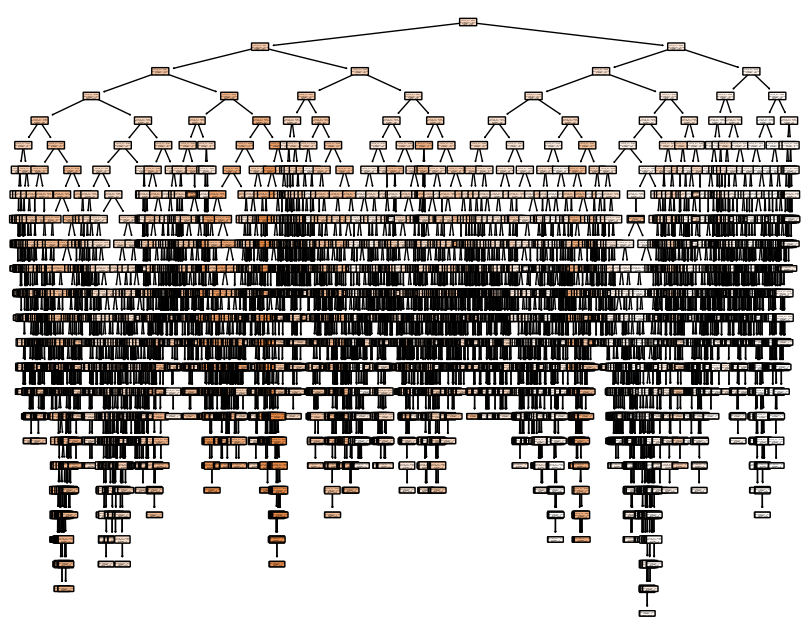
\includegraphics[width=1\linewidth]{HW4/images/tree1.png}
    \label{fig:enter-label}
\end{figure}

\begin{lstlisting}
from sklearn.tree import plot_tree
from sklearn.tree import export_text


# print(forest_r.estimators_) #list of decision trees in the ensemble

plt.figure(figsize=(10, 8))
plot_tree(first_tree_r, filled=True, feature_names=['feature_0', 'feature_1', ...], rounded=True, max_depth = 2)
plt.show()    
\end{lstlisting}

\begin{figure}[H]
    \centering
    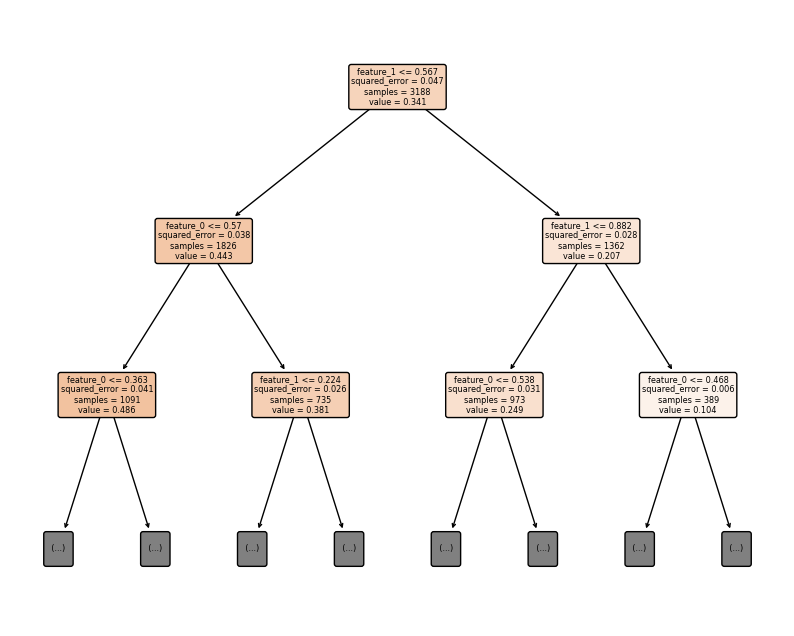
\includegraphics[width=1\linewidth]{HW4/images/tree2.png}
    \label{fig:enter-label}
\end{figure}

\end{Solution}

\begin{Problem*}[ii.]
 Why does the resulting image look like the way it does? What shape are the patches of color, and how are they arranged?
\end{Problem*}
\begin{Solution}

We chose to analyze the last image in the pruning process cell, with depth=10, min leaf=10, and sample=10. The image looks blocky because the decision trees within the forest are making predictions based on the average/majority color of the training samples within the region associated with a designated leaf node (or pixel) launched earlier. That's why it seems to have no wavy/smooth shapes.

\begin{lstlisting}[language=Python]

\end{lstlisting}
\end{Solution}

\section*{Written Exercises}

\setcounter{section}{0}
\section{Maximum Margin Classifiers.}
\setcounter{Problem}{0}
Suppose we are given \( n = 7 \) observations in \( d = 2 \) dimensions. For each observation, there is an associated class label.
\begin{center}
\begin{tabular}{ |c|c|c| }
\hline
\( x_1 \) & \( x_2 \) & y \\
\hline
3 & 4 & Red \\
2 & 2 & Red \\
4 & 4 & Red \\
1 & 4 & Red \\
2 & 1 & Blue \\
4 & 3 & Blue \\
4 & 1 & Blue \\
\hline
\end{tabular}
\end{center}
\begin{Problem*}[(a)]
Sketch the observations and the maximum-margin separating hyperplane.
\end{Problem*}

\begin{Solution}
\begin{figure}[H]
    \centering
    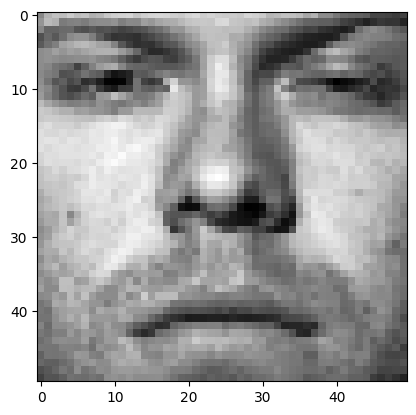
\includegraphics[width=1\linewidth]{HW4//images/image1.png}
    \caption{Sketch of the points and hyperplane}
    \label{fig:enter-label}
\end{figure}
\end{Solution}

\begin{Problem*}[(b)]
 Describe the classification rule for the maximal margin classifier. It should be something along the lines of ``Classify as Red if \( \beta_0 + \beta_1x_1 + \beta_2x_2 < 0 \), and classify to Blue otherwise.'' Provide the values for \( \beta_0, \beta_1, \) and \( \beta_2 \).
\end{Problem*}

\begin{Solution}
The classification rule for the maximal margin classifier is:

Classify as Red if \( \beta_0 + \beta_1x_1 + \beta_2x_2 < 0 \), and classify as Blue otherwise.

The values for the coefficients are:
\begin{itemize}
    \item \( \beta_0 = 1 \) 
    \item \( \beta_1 = -2 \)
    \item \( \beta_2 = 2 \) 
\end{itemize}

Therefore, the rule can be written as:

Classify as Red if \( 1 - 2x_1 + 2x_2 < 0 \), and classify as Blue otherwise.
\end{Solution}

\begin{Problem*}[(c)]
 On your sketch, indicate the margin for the maximal margin hyperplane.
\end{Problem*}

\begin{Solution}

\begin{figure}[H]
    \centering
    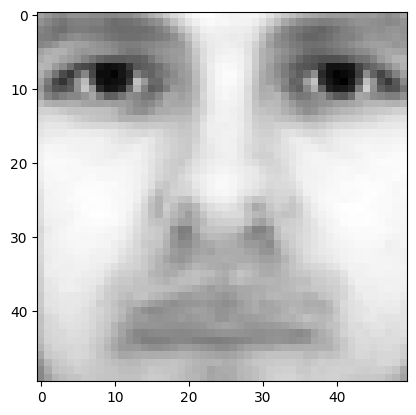
\includegraphics[width=1\linewidth]{HW4//images/image2.png}
    \caption{Sketch of the points and hyperplane}
    \label{fig:enter-label}
\end{figure}
The solid line represents the maximum-margin separating hyperplane found by the SVM.
The dashed lines are the margins of the hyperplane, which are equidistant from the closest points of the two classes (these points are the support vectors).
\end{Solution}

\begin{Problem*}[(d)]
 Indicate the support vectors for the maximal margin classifier.
\end{Problem*}

\begin{Solution}
The support vectors for the maximal margin classifier are the data points that are closest to the decision boundary, which are:
\begin{itemize}
    \item (2, 1) - Blue class
    \item (4, 3) - Blue class
    \item (2, 2) - Red class
    \item (4, 4) - Red class
\end{itemize}


These points are the ones that directly influence the position and orientation of the hyperplane.
\end{Solution}

\begin{Problem*}[(e)]
 Argue that a slight movement of the seventh observation would not affect the maximal margin hyperplane.
\end{Problem*}

\begin{Solution}
The maximal margin hyperplane in a Support Vector Machine (SVM) is defined by the support vectors, which are the data points that are closest to the decision boundary. These points are the critical elements that determine the position and orientation of the hyperplane. The hyperplane is computed in such a way that it maximizes the margin, which is the distance between the hyperplane and the nearest points from each class.

From the support vectors that we identified earlier, the seventh observation (with coordinates (4,1)) in the dataset is not one of the support vectors. This means that it is not one of the points that are closest to the decision boundary. As a result, a slight movement of this observation would not affect the maximal margin hyperplane, as long as it does not cross the decision boundary or become one of the new support vectors.

In SVMs, only support vectors are used to define the hyperplane. Other points (non-support vectors) have no influence on the hyperplane as long as they remain on their respective sides of the margin. Therefore, unless the movement of the seventh observation is substantial enough to make it a support vector or cause it to cross into the margin or the other class, the maximal margin hyperplane will remain unchanged.
\end{Solution}

\begin{Problem*}[(f)]
 Sketch a hyperplane that separates the data, but is not the maximum-margin separating hyperplane. Provide the equation for this hyperplane.
\end{Problem*}

\begin{Solution}
\begin{figure}[H]
    \centering
    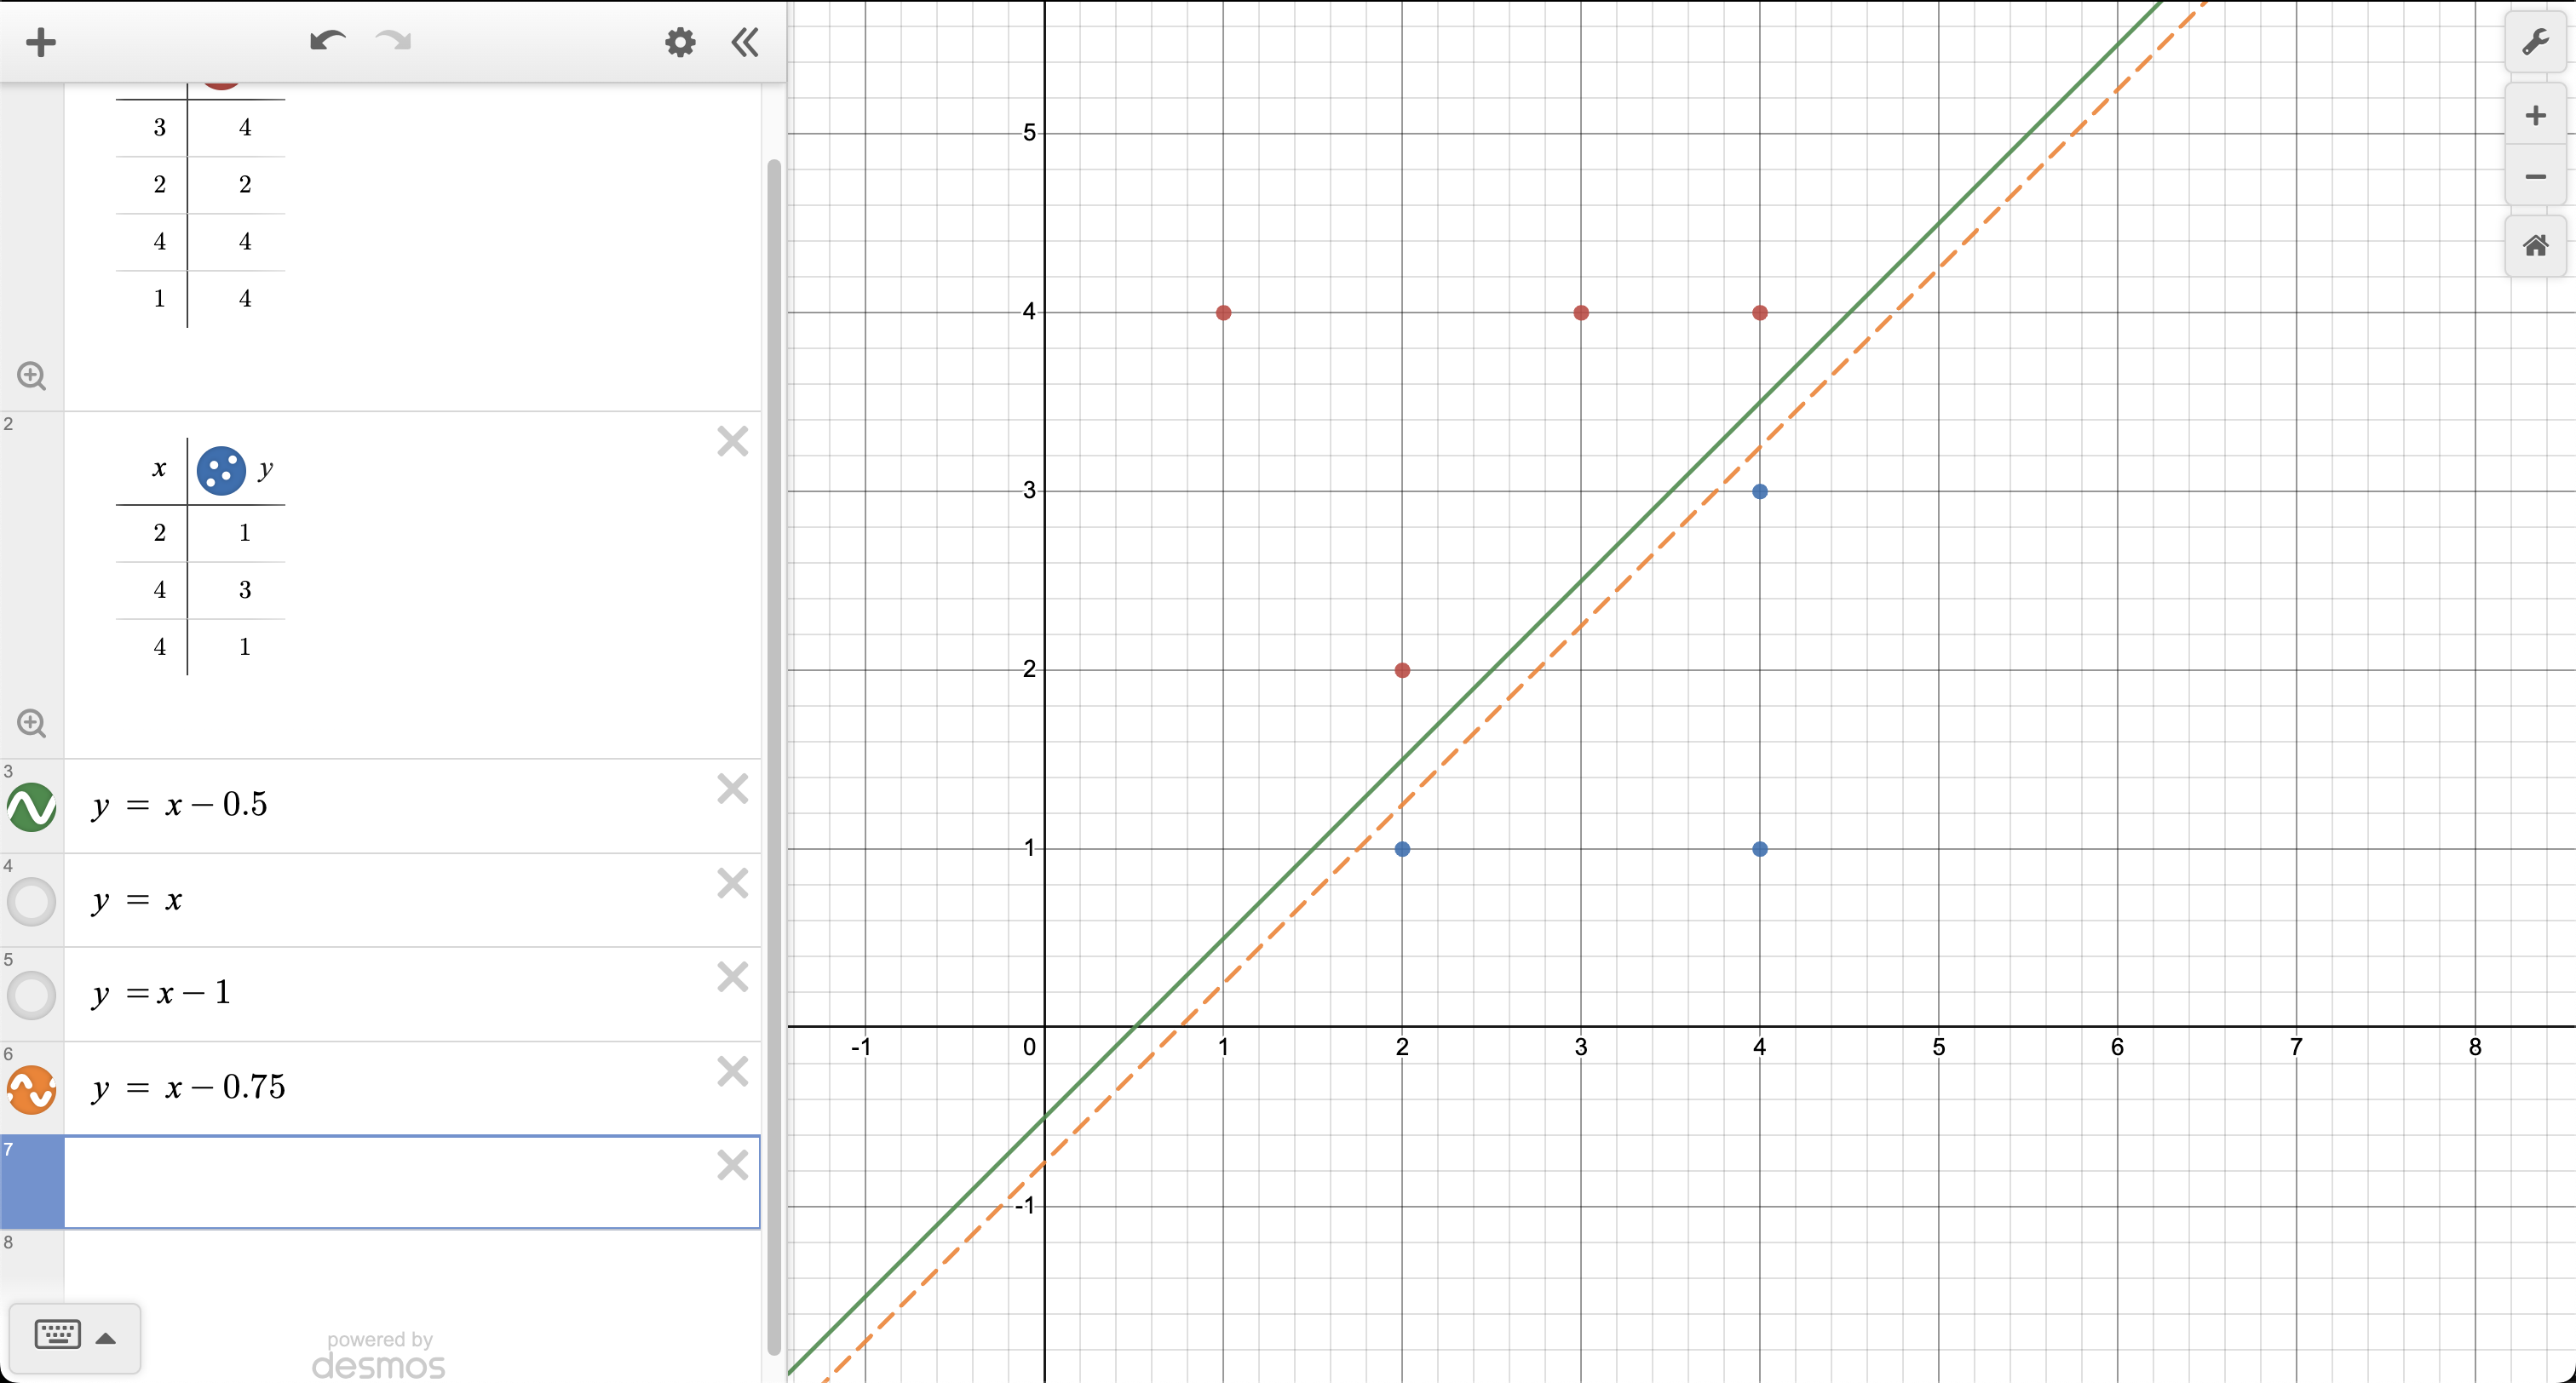
\includegraphics[width=1\linewidth]{HW4//images/image3.png}
    \caption{Not maximum-margin separating hyperplane}
    \label{fig:enter-label}
\end{figure}

The orange dashed line in the plot above represents a hyperplane that separates the data but is not the maximum-margin separating hyperplane. By slightly shifting the intercept of the original maximum-margin hyperplane, we have created a new hyperplane that still separates the classes but with a smaller margin.

The equation for this adjusted hyperplane can be given by:

\[ y = -2x_1 + 2x_2 + 0.75 \]

where \( \beta_0 \) (the adjusted intercept) is 0.75, \( \beta_1 \) remains -2, and \( \beta_2 \) remains 2.

This line still separates the red and blue points, but since it doesn't maximize the margin between the classes, it is not considered a maximum-margin hyperplane.

\end{Solution}

\begin{Problem*}[(g)]
 Draw an additional observation on the plot so that the two classes are no longer separable by a hyperplane.
\end{Problem*}

\begin{Solution}
\begin{figure}[H]
    \centering
    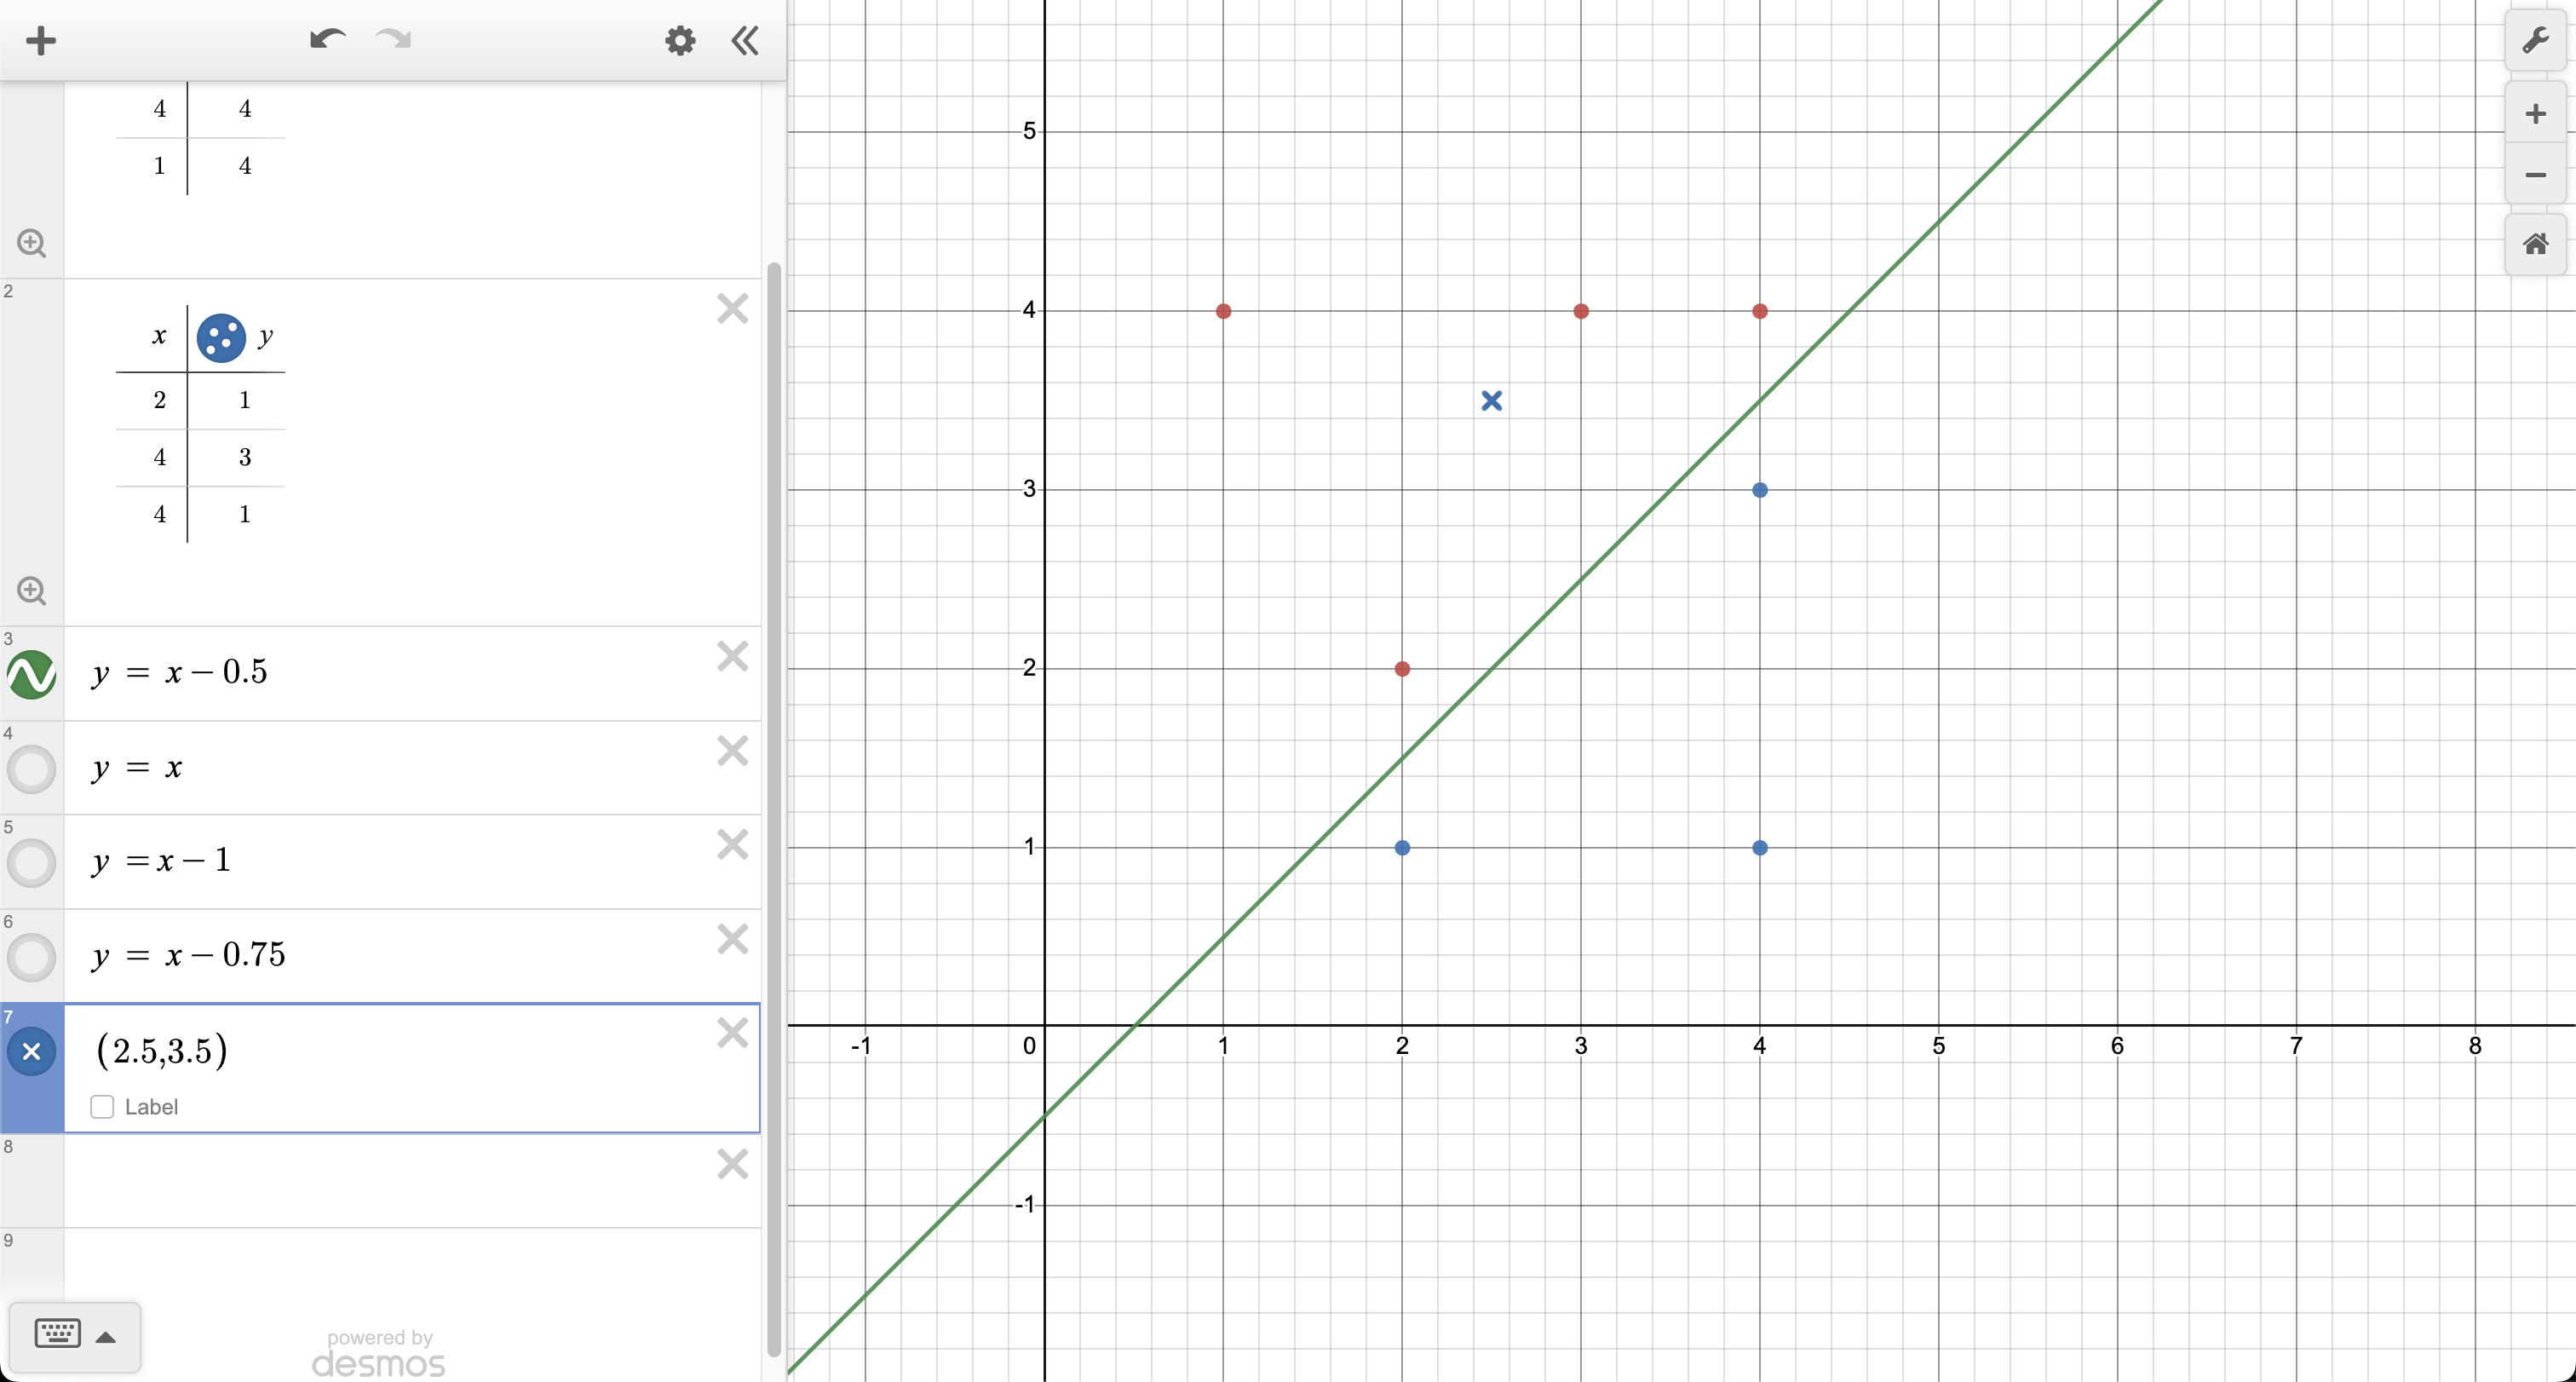
\includegraphics[width=1\linewidth]{HW4//images/image4.png}
    \caption{Inseparable Plot}
    \label{fig:enter-label}
\end{figure}
In the updated plot above, a new observation has been added (marked with an 'x'), which belongs to the blue class but is positioned among the red points. This new point makes it impossible to separate the two classes with a single straight hyperplane, as it violates the previous clear separation. The presence of this point within the margin of the red class means that any hyperplane trying to separate the two classes would either misclassify this new blue point or some of the red points, indicating that the dataset is no longer linearly separable.
\end{Solution}

\section{Ensemble Models}
In this question, we will get more hands-on experience using ensemble models. Throughout, suppose our inputs live in two-dimensional space. Formally, for all $\mathbf{x} \in \mathbb{R}^{2}$, let $\mathbf{x}_{1}$ and $\mathbf{x}_{2}$ be the first and second components of the input vector, respectively. Suppose we have a binary classification dataset consisting of four labeled datapoints, with labels $y^{(i)} \in\{0,1\}$:
\begin{figure}[H]
    \centering
    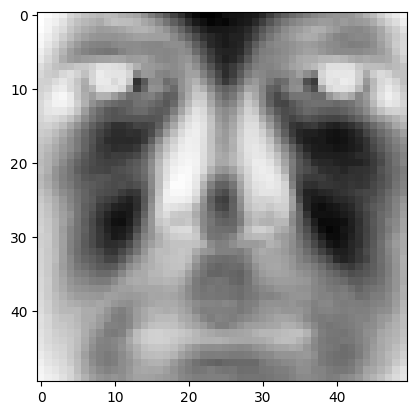
\includegraphics[width=1\linewidth]{HW4//images/image.png}
    \label{fig:enter-label}
\end{figure}

As you can see in the plot above, this dataset is diagonally linearly separable, meaning there is a diagonal linear decision boundary that will perfectly classify the points with label 1 (filled in black) and those with label 0 (not filled).

\begin{Problem*}[(a)]
 Let $g: \mathbb{R}^{2} \mapsto\{0,1\}$ be a binary classifier of the form $g(x)=\mathbf{1}\left\{\mathbf{x}_{j}>c\right\}$, where $\mathbf{1}$ is an indicator function (equal to one if its input is true and zero otherwise), $j \in\{1,2\}$ is a coordinate, and $c \in \mathbb{R}$ is a threshold value. In other words, the function $g$ looks at some coordinate $j$ of $\mathbf{x}$ and
returns one if it is greater than $c$, and zero otherwise. Note that we can view $g$ as a decision tree of depth one. We will refer to a $g$ of this form as a threshold function.

There exists an ensemble model $f(\mathbf{x})=\sum_{t=1}^{T} \alpha_{t} g_{t}\left(\mathbf{x}^{(i)}\right)$ consisting of a weighted average of $T$ threshold functions $g_{t}$ with weights given by $\alpha_{t} \in \mathbb{R}$ such that the training error of $f$ is zero (i.e., for all points $\mathbf{x}^{(i)}$ in the training set, $y^{(i)}=\mathbf{1}\left\{f\left(\mathbf{x}^{(i)}\right)>0.5\right\}$ ). In other words, we can ensemble shallow decision trees that represent only horizontal or vertical decision boundaries into a more expressive classifier with a diagonal decision boundary. Find the functions $g_{t}$ and the weights $\alpha_{t}$ that yield an ensemble $f$ with a classification error of zero on the training set.

(Hint: there exists a solution with $T=3$. Also, the weights can all be equal.)
\end{Problem*} 

\begin{Solution}

\begin{figure}[H]
    \centering
    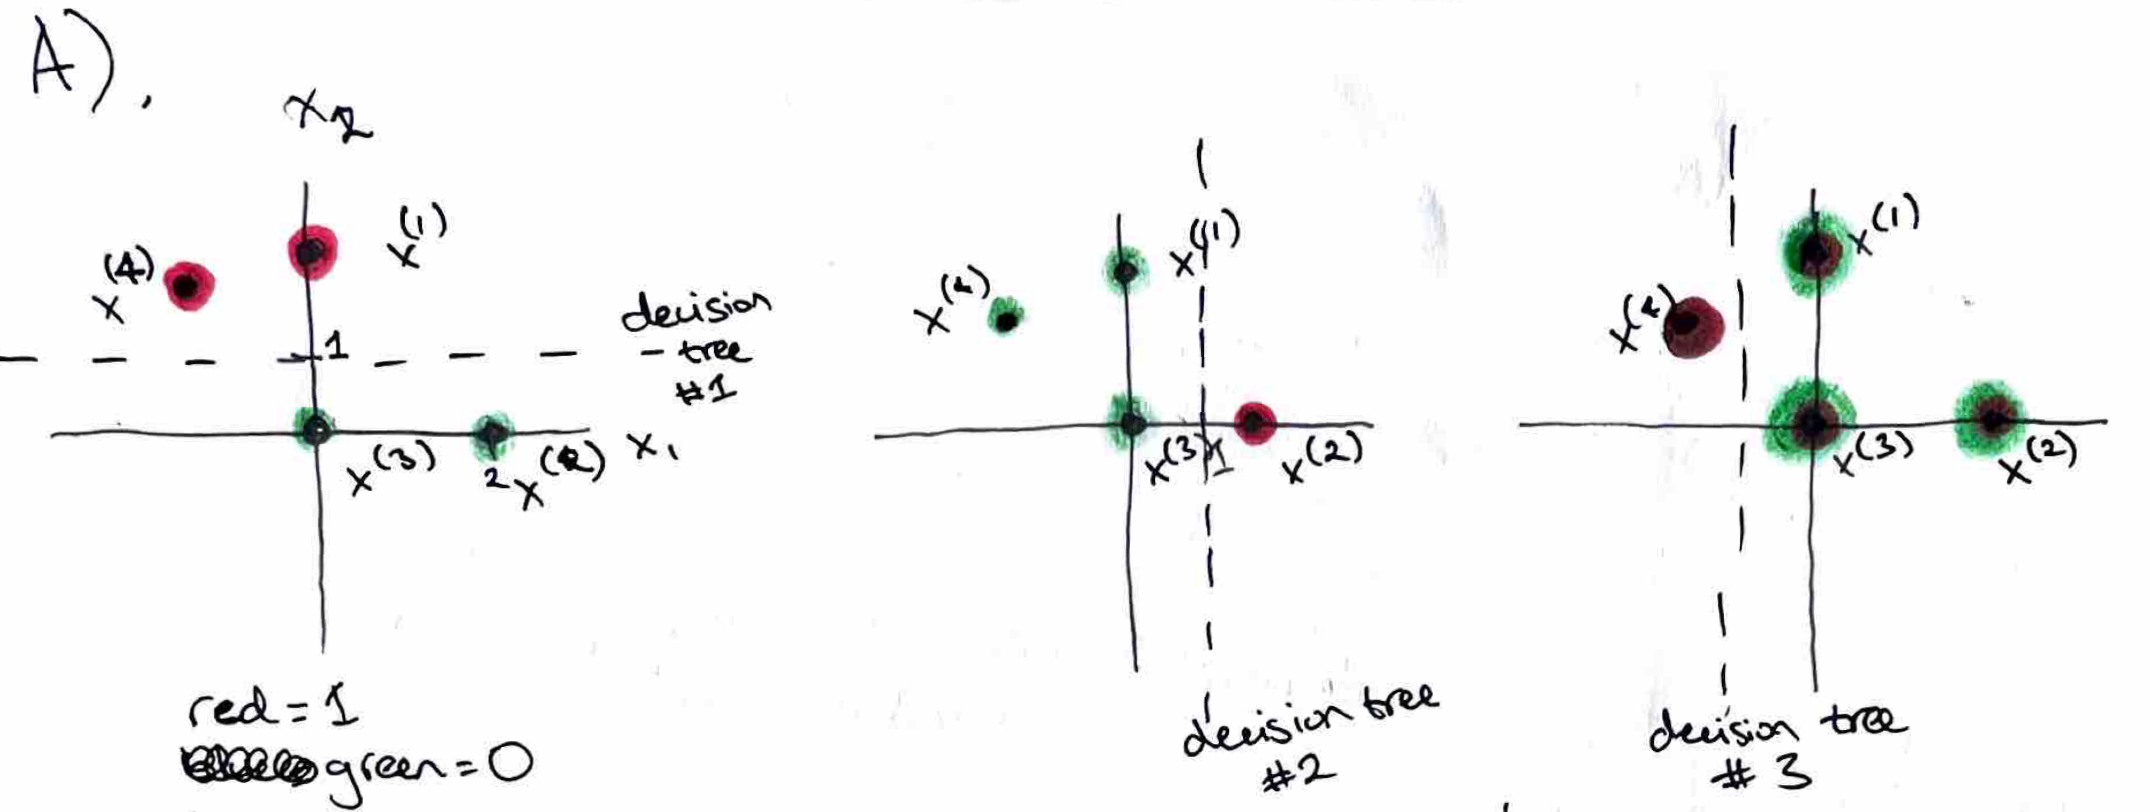
\includegraphics[width=1\linewidth]{HW4//images/2a-1.png}
\end{figure}
\begin{figure}[H]
    \centering
    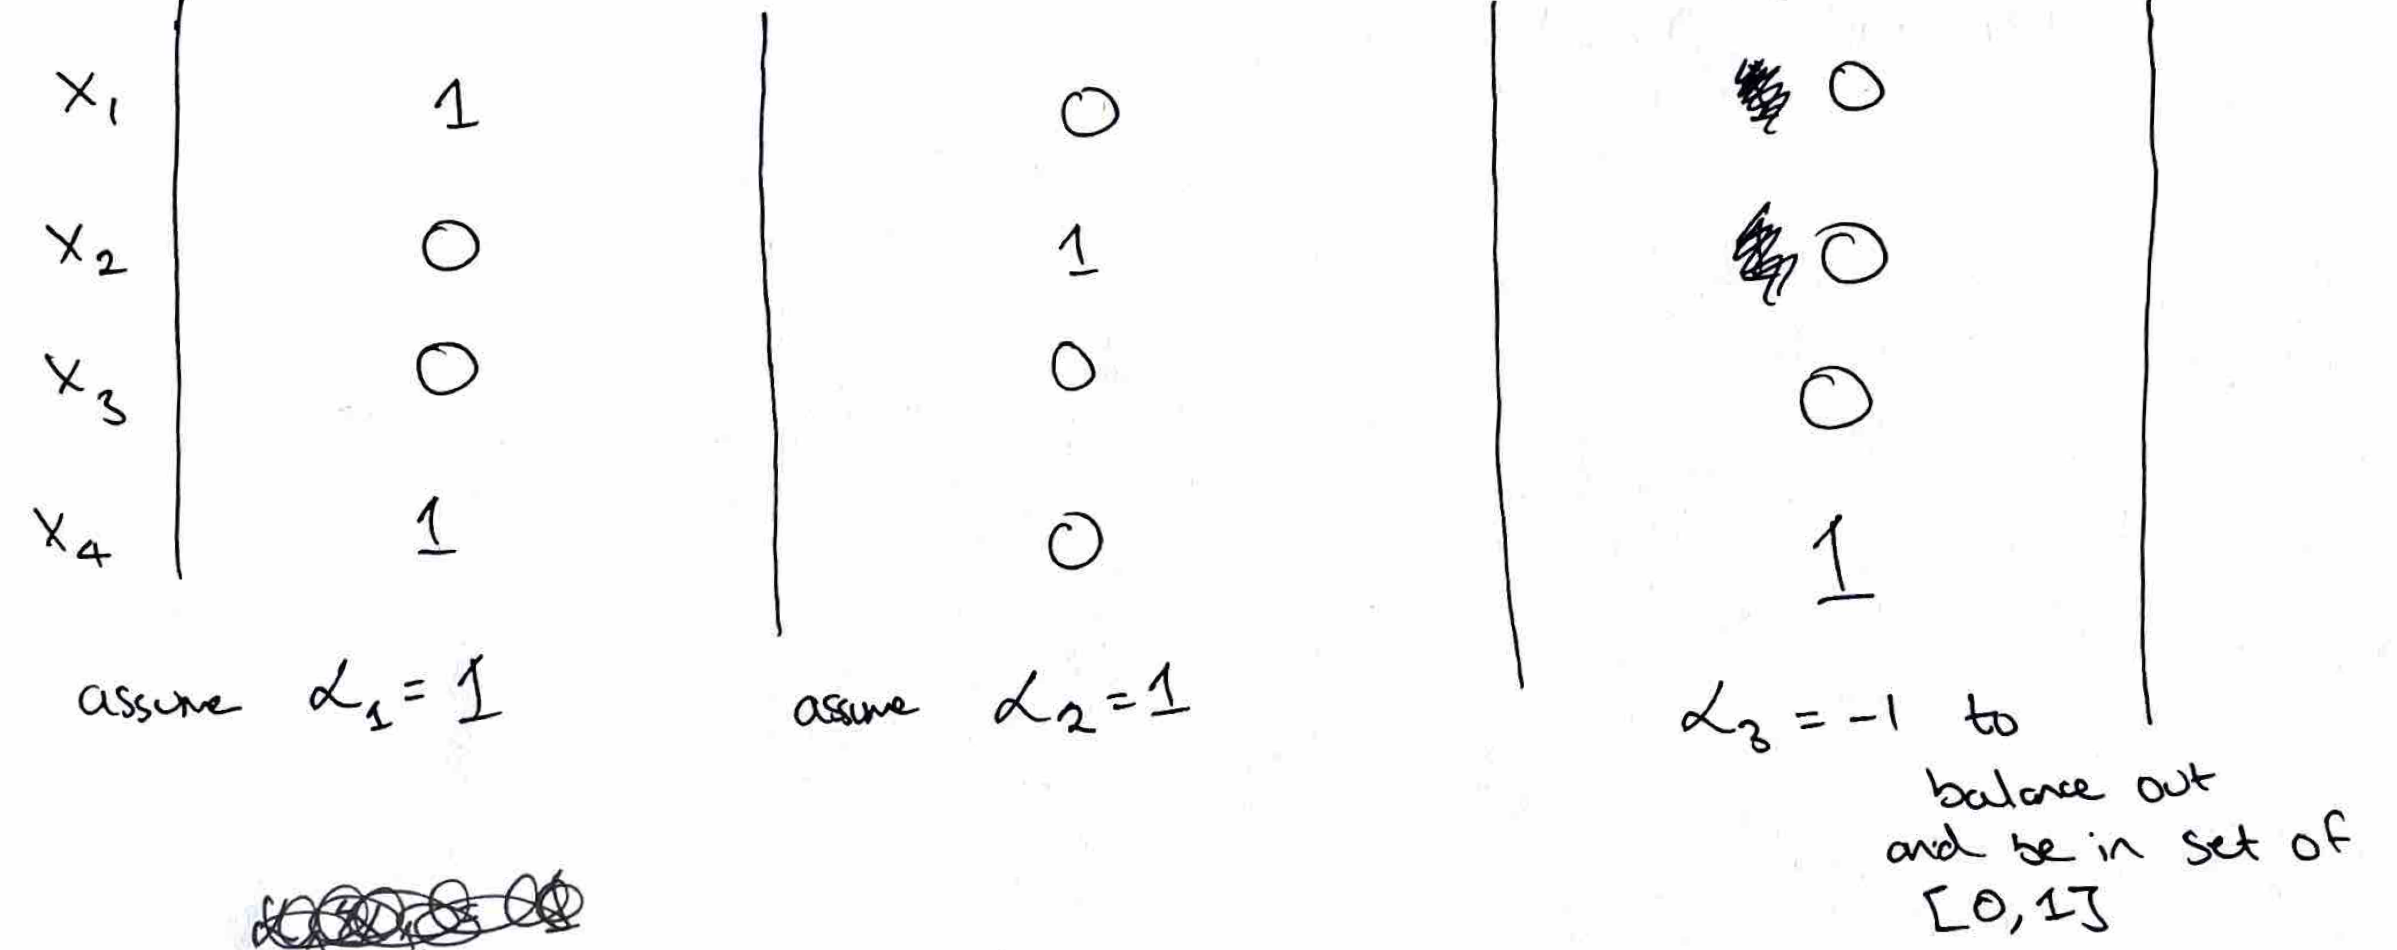
\includegraphics[width=1\linewidth]{HW4//images/2a-2.png}
\end{figure}
\begin{figure}[H]
    \centering
    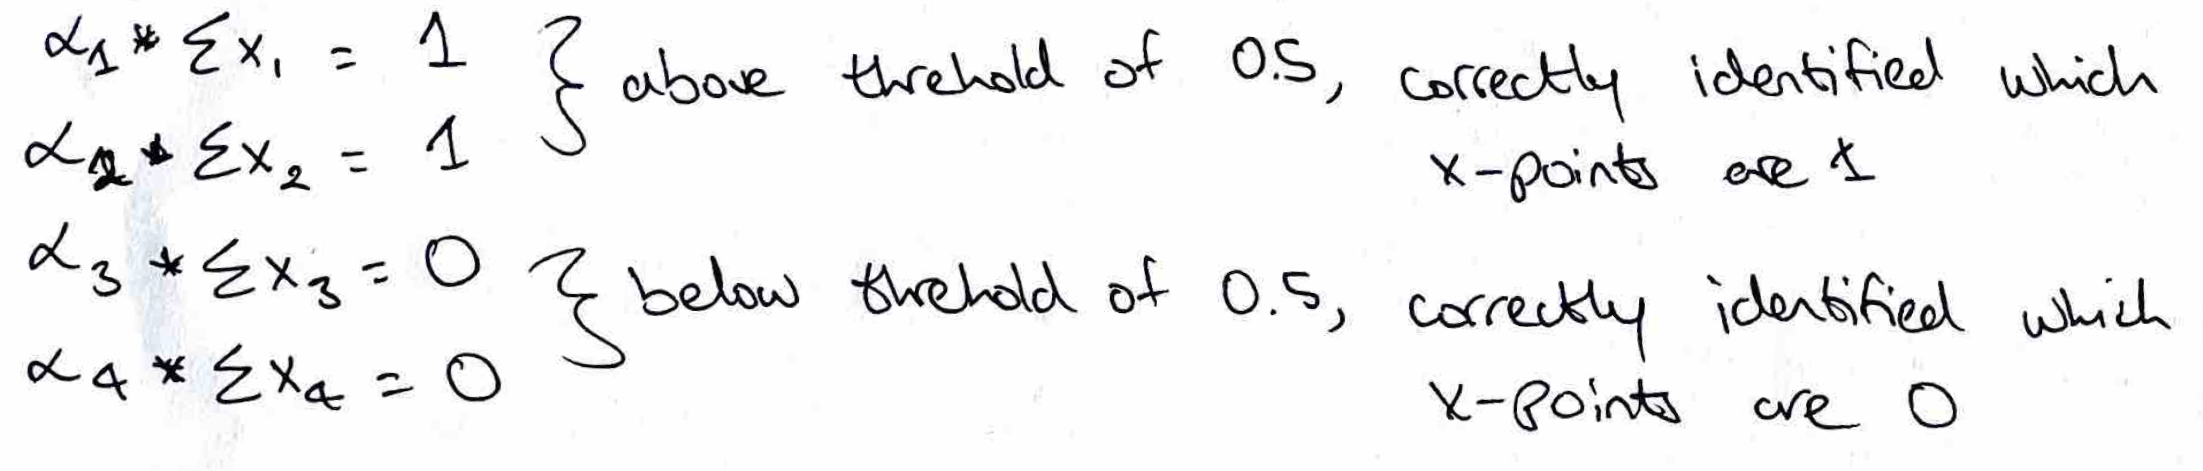
\includegraphics[width=1\linewidth]{HW4//images/2a-3.png}
\end{figure}
\begin{figure}[H]
    \centering
    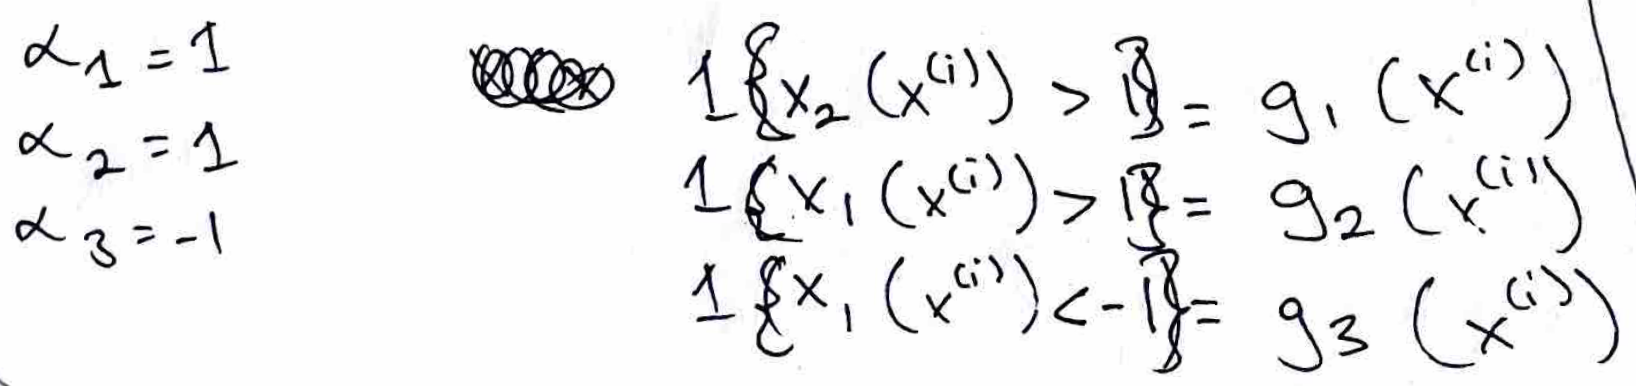
\includegraphics[width=0.75\linewidth]{HW4//images/2a-4.png}
\end{figure}
\end{Solution}

\begin{Problem*}[(b)]
 On the original plot above or on a duplicate, draw the decision boundary of this ensemble and clearly indicate on which side your ensemble would predict a label of +1 or 0.
\end{Problem*} 

\begin{Solution}

\begin{figure}[H]
    \centering
    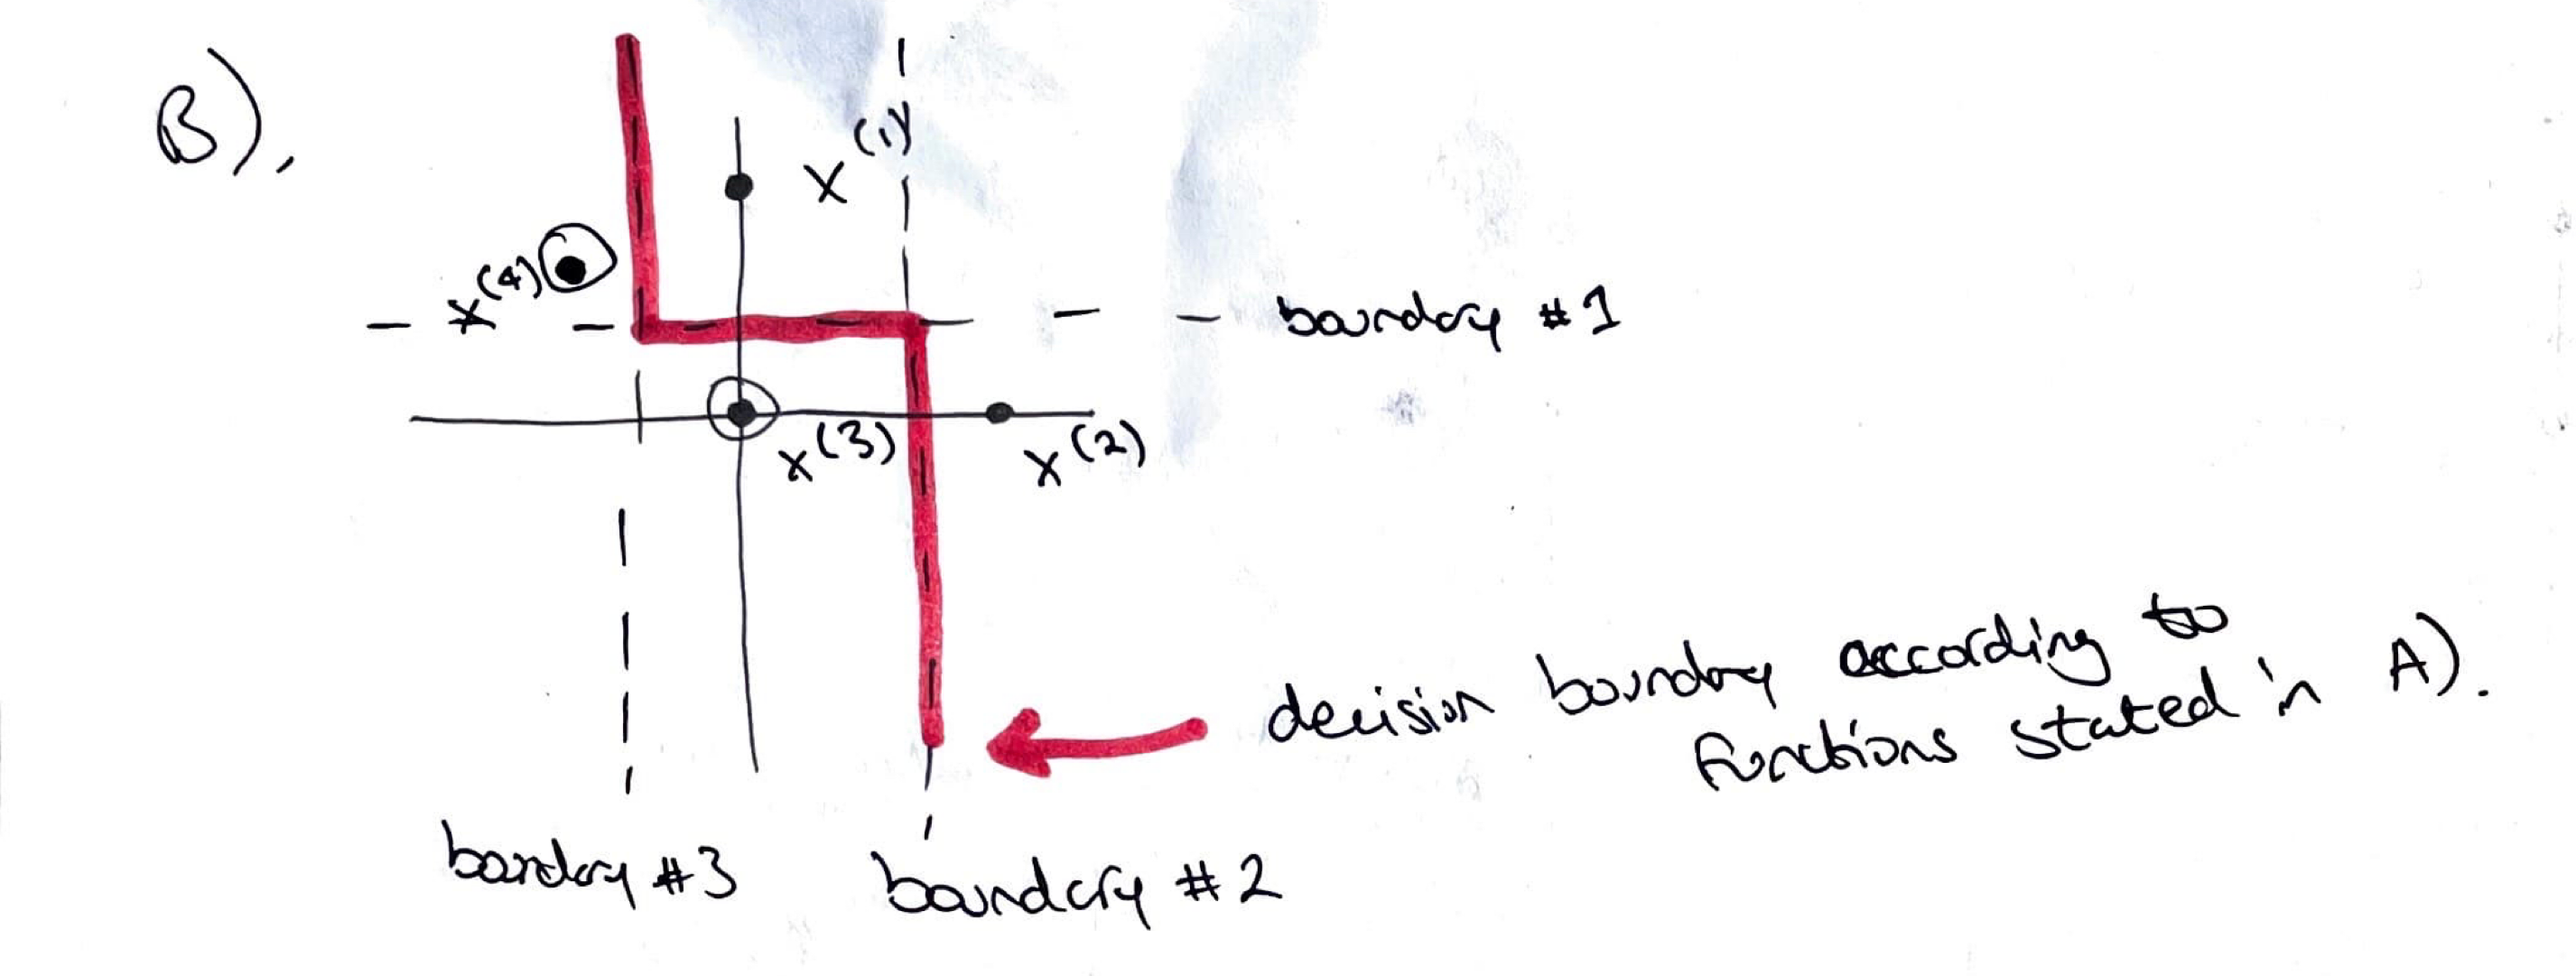
\includegraphics[width=1\linewidth]{HW4//images/2b.png}
\end{figure}

\end{Solution}

%%%%%%%%%%%%%%%%%%%%%%%%%%%%%%%%%%%%%%%%%%%%%%%%%%%%%%%%%%%%%%%%%%
%Complete the assignment now
\end{document}

%%%%%%%%%%%%%%%%%%%%%%%%%%%%%%%%%%%%%%%%%%%%%%%%%%%%%%%%%%%%%%%%%%
%%%%%%%%%%%%%%%%%%%%%%%%%%%%%%%%%%%%%%%%%%%%%%%%%%%%%%%%%%%%%%%%%%
